%%
%% Beginning of file 'sample62.tex'
%%
%% Modified 2018 January
%%
%% This is a sample manuscript marked up using the
%% AASTeX v6.2 LaTeX 2e macros.
%%
%% AASTeX is now based on Alexey Vikhlinin's emulateapj.cls 
%% (Copyright 2000-2015).  See the classfile for details.

%% AASTeX requires revtex4-1.cls (http://publish.aps.org/revtex4/) and
%% other external packages (latexsym, graphicx, amssymb, longtable, and epsf).
%% All of these external packages should already be present in the modern TeX 
%% distributions.  If not they can also be obtained at www.ctan.org.

%% The first piece of markup in an AASTeX v6.x document is the \documentclass
%% command. LaTeX will ignore any data that comes before this command. The 
%% documentclass can take an optional argument to modify the output style.
%% The command below calls the preprint style  which will produce a tightly 
%% typeset, one-column, single-spaced document.  It is the default and thus
%% does not need to be explicitly stated.
%%
%%
%% using aastex version 6.2
\documentclass[twocolumn]{aastex62}

%% The default is a single spaced, 10 point font, single spaced article.
%% There are 5 other style options available via an optional argument. They
%% can be envoked like this:
%%
%% \documentclass[argument]{aastex62}
%% 
%% where the layout options are:
%%
%%  twocolumn   : two text columns, 10 point font, single spaced article.
%%                This is the most compact and represent the final published
%%                derived PDF copy of the accepted manuscript from the publisher
%%  manuscript  : one text column, 12 point font, double spaced article.
%%  preprint    : one text column, 12 point font, single spaced article.  
%%  preprint2   : two text columns, 12 point font, single spaced article.
%%  modern      : a stylish, single text column, 12 point font, article with
%% 		  wider left and right margins. This uses the Daniel
%% 		  Foreman-Mackey and David Hogg design.
%%  RNAAS       : Preferred style for Research Notes which are by design 
%%                lacking an abstract and brief. DO NOT use \begin{abstract}
%%                and \end{abstract} with this style.
%%
%% Note that you can submit to the AAS Journals in any of these 6 styles.
%%
%% There are other optional arguments one can envoke to allow other stylistic
%% actions. The available options are:
%%
%%  astrosymb    : Loads Astrosymb font and define \astrocommands. 
%%  tighten      : Makes baselineskip slightly smaller, only works with 
%%                 the twocolumn substyle.
%%  times        : uses times font instead of the default
%%  linenumbers  : turn on lineno package.
%%  trackchanges : required to see the revision mark up and print its output
%%  longauthor   : Do not use the more compressed footnote style (default) for 
%%                 the author/collaboration/affiliations. Instead print all
%%                 affiliation information after each name. Creates a much
%%                 long author list but may be desirable for short author papers
%%
%% these can be used in any combination, e.g.
%%
%% \documentclass[twocolumn,linenumbers,trackchanges]{aastex62}
%%
%% AASTeX v6.* now includes \hyperref support. While we have built in specific
%% defaults into the classfile you can manually override them with the
%% \hypersetup command. For example,
%%
%%\hypersetup{linkcolor=red,citecolor=green,filecolor=cyan,urlcolor=magenta}
%%
%% will change the color of the internal links to red, the links to the
%% bibliography to green, the file links to cyan, and the external links to
%% magenta. Additional information on \hyperref options can be found here:
%% https://www.tug.org/applications/hyperref/manual.html#x1-40003
%%
%% If you want to create your own macros, you can do so
%% using \newcommand. Your macros should appear before
%% the \begin{document} command.
%%
\newcommand{\vdag}{(v)^\dagger}
\newcommand\aastex{AAS\TeX}
\newcommand\latex{La\TeX}
\usepackage{float}
\usepackage{wrapfig}

%% Tells LaTeX to search for image files in the 
%% current directory as well as in the figures/ folder.
\graphicspath{{./}{figures/}}

%% Reintroduced the \received and \accepted commands from AASTeX v5.2
\received{}
\revised{}
\accepted{\today}
%% Command to document which AAS Journal the manuscript was submitted to.
%% Adds "Submitted to " the arguement.
\submitjournal{ApJ}

%% Mark up commands to limit the number of authors on the front page.
%% Note that in AASTeX v6.2 a \collaboration call (see below) counts as
%% an author in this case.
%
%\AuthorCollaborationLimit=3
%
%% Will only show Schwarz, Muench and "the AAS Journals Data Scientist 
%% collaboration" on the front page of this example manuscript.
%%
%% Note that all of the author will be shown in the published article.
%% This feature is meant to be used prior to acceptance to make the
%% front end of a long author article more manageable. Please do not use
%% this functionality for manuscripts with less than 20 authors. Conversely,
%% please do use this when the number of authors exceeds 40.
%%
%% Use \allauthors at the manuscript end to show the full author list.
%% This command should only be used with \AuthorCollaborationLimit is used.

%% The following command can be used to set the latex table counters.  It
%% is needed in this document because it uses a mix of latex tabular and
%% AASTeX deluxetables.  In general it should not be needed.
%\setcounter{table}{1}

%%%%%%%%%%%%%%%%%%%%%%%%%%%%%%%%%%%%%%%%%%%%%%%%%%%%%%%%%%%%%%%%%%%%%%%%%%%%%%%%
%%
%% The following section outlines numerous optional output that
%% can be displayed in the front matter or as running meta-data.
%%
%% If you wish, you may supply running head information, although
%% this information may be modified by the editorial offices.
\shorttitle{SED/Stellar Mass Draft}
\shortauthors{S. Lower}
%%
%% You can add a light gray and diagonal water-mark to the first page 
%% with this command:
% \watermark{text}
%% where "text", e.g. DRAFT, is the text to appear.  If the text is 
%% long you can control the water-mark size with:
%  \setwatermarkfontsize{dimension}
%% where dimension is any recognized LaTeX dimension, e.g. pt, in, etc.
%%
%%%%%%%%%%%%%%%%%%%%%%%%%%%%%%%%%%%%%%%%%%%%%%%%%%%%%%%%%%%%%%%%%%%%%%%%%%%%%%%%

%% This is the end of the preamble.  Indicate the beginning of the
%% manuscript itself with \begin{document}.

\begin{document}

\title{How Well Can We Measure the Stellar Mass of Galaxies? \\ Ground-Truthing SED Fitting Methods with Cosmological Simulations
}

%% LaTeX will automatically break titles if they run longer than
%% one line. However, you may use \\ to force a line break if
%% you desire. In v6.2 you can include a footnote in the title.

%% A significant change from earlier AASTEX versions is in the structure for 
%% calling author and affilations. The change was necessary to implement 
%% autoindexing of affilations which prior was a manual process that could 
%% easily be tedious in large author manuscripts.
%%
%% The \author command is the same as before except it now takes an optional
%% arguement which is the 16 digit ORCID. The syntax is:
%% \author[xxxx-xxxx-xxxx-xxxx]{Author Name}
%%
%% This will hyperlink the author name to the author's ORCID page. Note that
%% during compilation, LaTeX will do some limited checking of the format of
%% the ID to make sure it is valid.
%%
%% Use \affiliation for affiliation information. The old \affil is now aliased
%% to \affiliation. AASTeX v6.2 will automatically index these in the header.
%% When a duplicate is found its index will be the same as its previous entry.
%%
%% Note that \altaffilmark and \altaffiltext have been removed and thus 
%% can not be used to document secondary affiliations. If they are used latex
%% will issue a specific error message and quit. Please use multiple 
%% \affiliation calls for to document more than one affiliation.
%%
%% The new \altaffiliation can be used to indicate some secondary information
%% such as fellowships. This command produces a non-numeric footnote that is
%% set away from the numeric \affiliation footnotes.  NOTE that if an
%% \altaffiliation command is used it must come BEFORE the \affiliation call,
%% right after the \author command, in order to place the footnotes in
%% the proper location.
%%
%% Use \email to set provide email addresses. Each \email will appear on its
%% own line so you can put multiple email address in one \email call. A new
%% \correspondingauthor command is available in V6.2 to identify the
%% corresponding author of the manuscript. It is the author's responsibility
%% to make sure this name is also in the author list.
%%
%% While authors can be grouped inside the same \author and \affiliation
%% commands it is better to have a single author for each. This allows for
%% one to exploit all the new benefits and should make book-keeping easier.
%%
%% If done correctly the peer review system will be able to
%% automatically put the author and affiliation information from the manuscript
%% and save the corresponding author the trouble of entering it by hand.

%co authors: desika, joel, ben, charlie, romeel, others?
\author{Sidney Lower}
\affil{University of Florida}



%% Note that the \and command from previous versions of AASTeX is now
%% depreciated in this version as it is no longer necessary. AASTeX 
%% automatically takes care of all commas and "and"s between authors names.

%% AASTeX 6.2 has the new \collaboration and \nocollaboration commands to
%% provide the collaboration status of a group of authors. These commands 
%% can be used either before or after the list of corresponding authors. The
%% argument for \collaboration is the collaboration identifier. Authors are
%% encouraged to surround collaboration identifiers with ()s. The 
%% \nocollaboration command takes no argument and exists to indicate that
%% the nearby authors are not part of surrounding collaborations.

%% Mark off the abstract in the ``abstract'' environment. 
\begin{abstract}

Of the many assumptions that go into modeling the spectral energy distribution (SED) of a galaxy, the star formation history and dust attenuation law dominate the uncertainty in stellar mass and star formation rate recovery. Classically, star formation histories (SFHs) are modeled with parameterized functional forms, but these forms are unlikely to capture the true diversity of galaxy SFHs and may impose systematic uncertainties and biases on results. Recently, non-parametric SFH models have shown promise in marginalizing over some of these uncertainties. Here, we examine the efficacy of these SFHs by ground-truthing them against high-res cosmological hydrodynamic galaxy formation simulations. We demonstrate that stellar masses can be estimated with greatly improved accuracy over traditional SFH forms, with uncertainties falling below the inescapable ‘factor of 2’ that has historically plagued stellar mass estimates. We also demonstrate the impact on our understanding of the evolution of the unexplained mismatch between the theoretical and observed SFR-M* relation in galaxies, with improved estimates of both stellar ages and star formation rates. 

\end{abstract}

%% Keywords should appear after the \end{abstract} command. 
%% See the online documentation for the full list of available subject
%% keywords and the rules for their use.
\keywords{}

%% From the front matter, we move on to the body of the paper.
%% Sections are demarcated by \section and \subsection, respectively.
%% Observe the use of the LaTeX \label
%% command after the \subsection to give a symbolic KEY to the
%% subsection for cross-referencing in a \ref command.
%% You can use LaTeX's \ref and \label commands to keep track of
%% cross-references to sections, equations, tables, and figures.
%% That way, if you change the order of any elements, LaTeX will
%% automatically renumber them.
%%
%% We recommend that authors also use the natbib \citep
%% and \citet commands to identify citations.  The citations are
%% tied to the reference list via symbolic KEYs. The KEY corresponds
%% to the KEY in the \bibitem in the reference list below. 

\section{Introduction} \label{sec:intro}

With the numerous large volume and panchromatic galaxy surveys available, the ability to accurately estimate the physical quantities of those galaxies is important for our understanding of galaxy formation and evolution. Modeling the ultraviolet (UV) to infrared (IR) spectral energy distributions (SEDs) is one of the main diagnostics used to understand the physical characteristics of galaxies, such as stellar mass, star formation rates, and the attenuation of stellar light by dust. The efficacy of SED modelling techniques is not well tested, at least systematically (see reviews by \cite{conroy_modeling_2013}; \cite{walcher_fitting_2011}). The derivation of galaxy physical properties, especially at high-redshift, is also highly sensitive to the SED modeling technique and the level of accuracy by which one can derive these properties is still unknown \citep{hayward_should_2015}. Comparisons between SED models and fitting codes tend to highlight the systematic uncertainties that plague models for stellar evolution, star formation history, and dust attenuation (\cite{hunt_comprehensive_2019}; \cite{mitchell_how_2013}; \cite{pforr_recovering_2012}), but without a way to ground-truth these results, we cannot know for sure how accurate these models are. 


The necessity of SED modeling lies in our ability to transform the observed light from a galaxy into physical properties like stellar mass. To estimate stellar mass, numerous assumptions must be made even prior to fitting an SED model to observed data. These assumptions - IMF, star formation history (SFH), dust attenuation curve - all affect the estimated stellar mass in multiple ways and the uncertainties associated with them. The estimated stellar mass relies on the ability of these models to accurately pinpoint the precise combination of physical processes. The degeneracies at work between parameters like stellar age and reddening from dust attenuation, along with the fact that typical observations only weakly constrain the SFH, make it a challenge to accurately model the observed light from a galaxy. Therefore, any improvement in our understanding of the affects that the models have on the output physical parameters (stellar mass) will lead to less confusion in the fitting process. 

Presently, we are interested in the affect of a particular star formation history model on the derived stellar mass of a galaxy. The most common models for SFH are parametric, i.e. they are described by some functional form and the parameters varied in the SED fit describe that functional form. Examples include the tau and delayed-tau models, which model the SFH as exponentially declining with some characteristic e-folding time. Although these models are computationally efficient, the restricted nature of the functional forms cannot hope to reproduce the diversity seen in true galaxy SFHs. Additionally, the physical properties estimated from these parametric SFHs can be severely biased by the imposed functional form and the indirect influence of the SFH parameter priors, causing incorrect estimations as well as underestimated uncertainties. As explored in \cite{carnall_how_2018}, the affect of changing the prior distributions on the model parameters is almost as significant as using an entirely different SFH model. Nonetheless, SED modeling done in the literature typically assumes a parametric form for the SFH. An example is the estimation of stellar masses of high redshift dusty galaxies. \cite{michalowski_stellar_2012} found that the assumed star formation history model had the largest affect on the uncertainity in the estimated stellar masses for observations of SMGs from the literature. \cite{dudzeviciute_alma_2019} found that the difference between estimated stellar masses predicted by \texttt{MAGPHYS} and true stellar masses for galaxies from the EAGLE simulation was close to 0.5 dex, consistent with the uncertainties in SMG stellar mass estimates and attributed to the SFH model used. 

Non-parametric SFH models have recently been shown to have the flexibility to reproduce the variation in SFHs seen in observations and cosmological simulations. This flexibility means that the SFHs are not biased towards any direction regarding stellar mass, whereas delayed-tau models have been shown to systematically underestimate stellar masses. These SFH models are non-parametric in the sense that they are not restricted to a certain functional form. Some non-parametric SFHs are modeled as a function of families of SFHs that effectively cover the space of all physical SFHs, as developed in \cite{iyer_reconstruction_2017} and improved upon in \cite{iyer_non-parametric_2019} with the Dense Basis method. Other methods go a step further and model the SFH of a galaxy as multiple bins of constant star formation rate, effectively removing any constraints from a functional form, as devloped in \cite{leja_deriving_2017} and expanded and improved upon in \cite{leja_how_2018} and \cite{leja_older_2019}. These models are described by priors on both the shape and normalization of the SFH. The shape of the SFH is informed by a certain prior and the overall normalization of the SFH informed by another, so that each component is effectively independent of the other. As described in detail in the Section  3.1.2 and 3.1.3, the two priors we considered for the fractional masses formed (controlling the shape of the SFH) are the Dirichlet and continuity prior distributions. The overall mass normalization is informed by a stellar mass-stellar metallicity prior via \cite{gallazzi_ages_2005}.   

An important avenue to explore is the ability of these non-parametric SFHs to recover both the stellar mass of a galaxy and the true SFH. To that end, we have used 'observations' of galaxies from cosmological simulations to both test and tune the parameters used to estimate these quantities. As opposed to conducting comparisons between various SED models and codes with observational data, we instead check the accuracy of a limited set of SED models, specifically two non-parametric SFH models from \cite{leja_how_2018}, against galaxies from the \texttt{simba} cosmological simulation, focusing on the stellar mass predictions made by the SED model. We We also compare the abilities of the non-parametric SFH models to the traditional parametric forms used and show that the non-parametric models are able to recover the observed star forming main sequence with much better accuracy.  



\section{\texttt{simba} Cosmological Simulation} 


\begin{figure*}
    \centering
    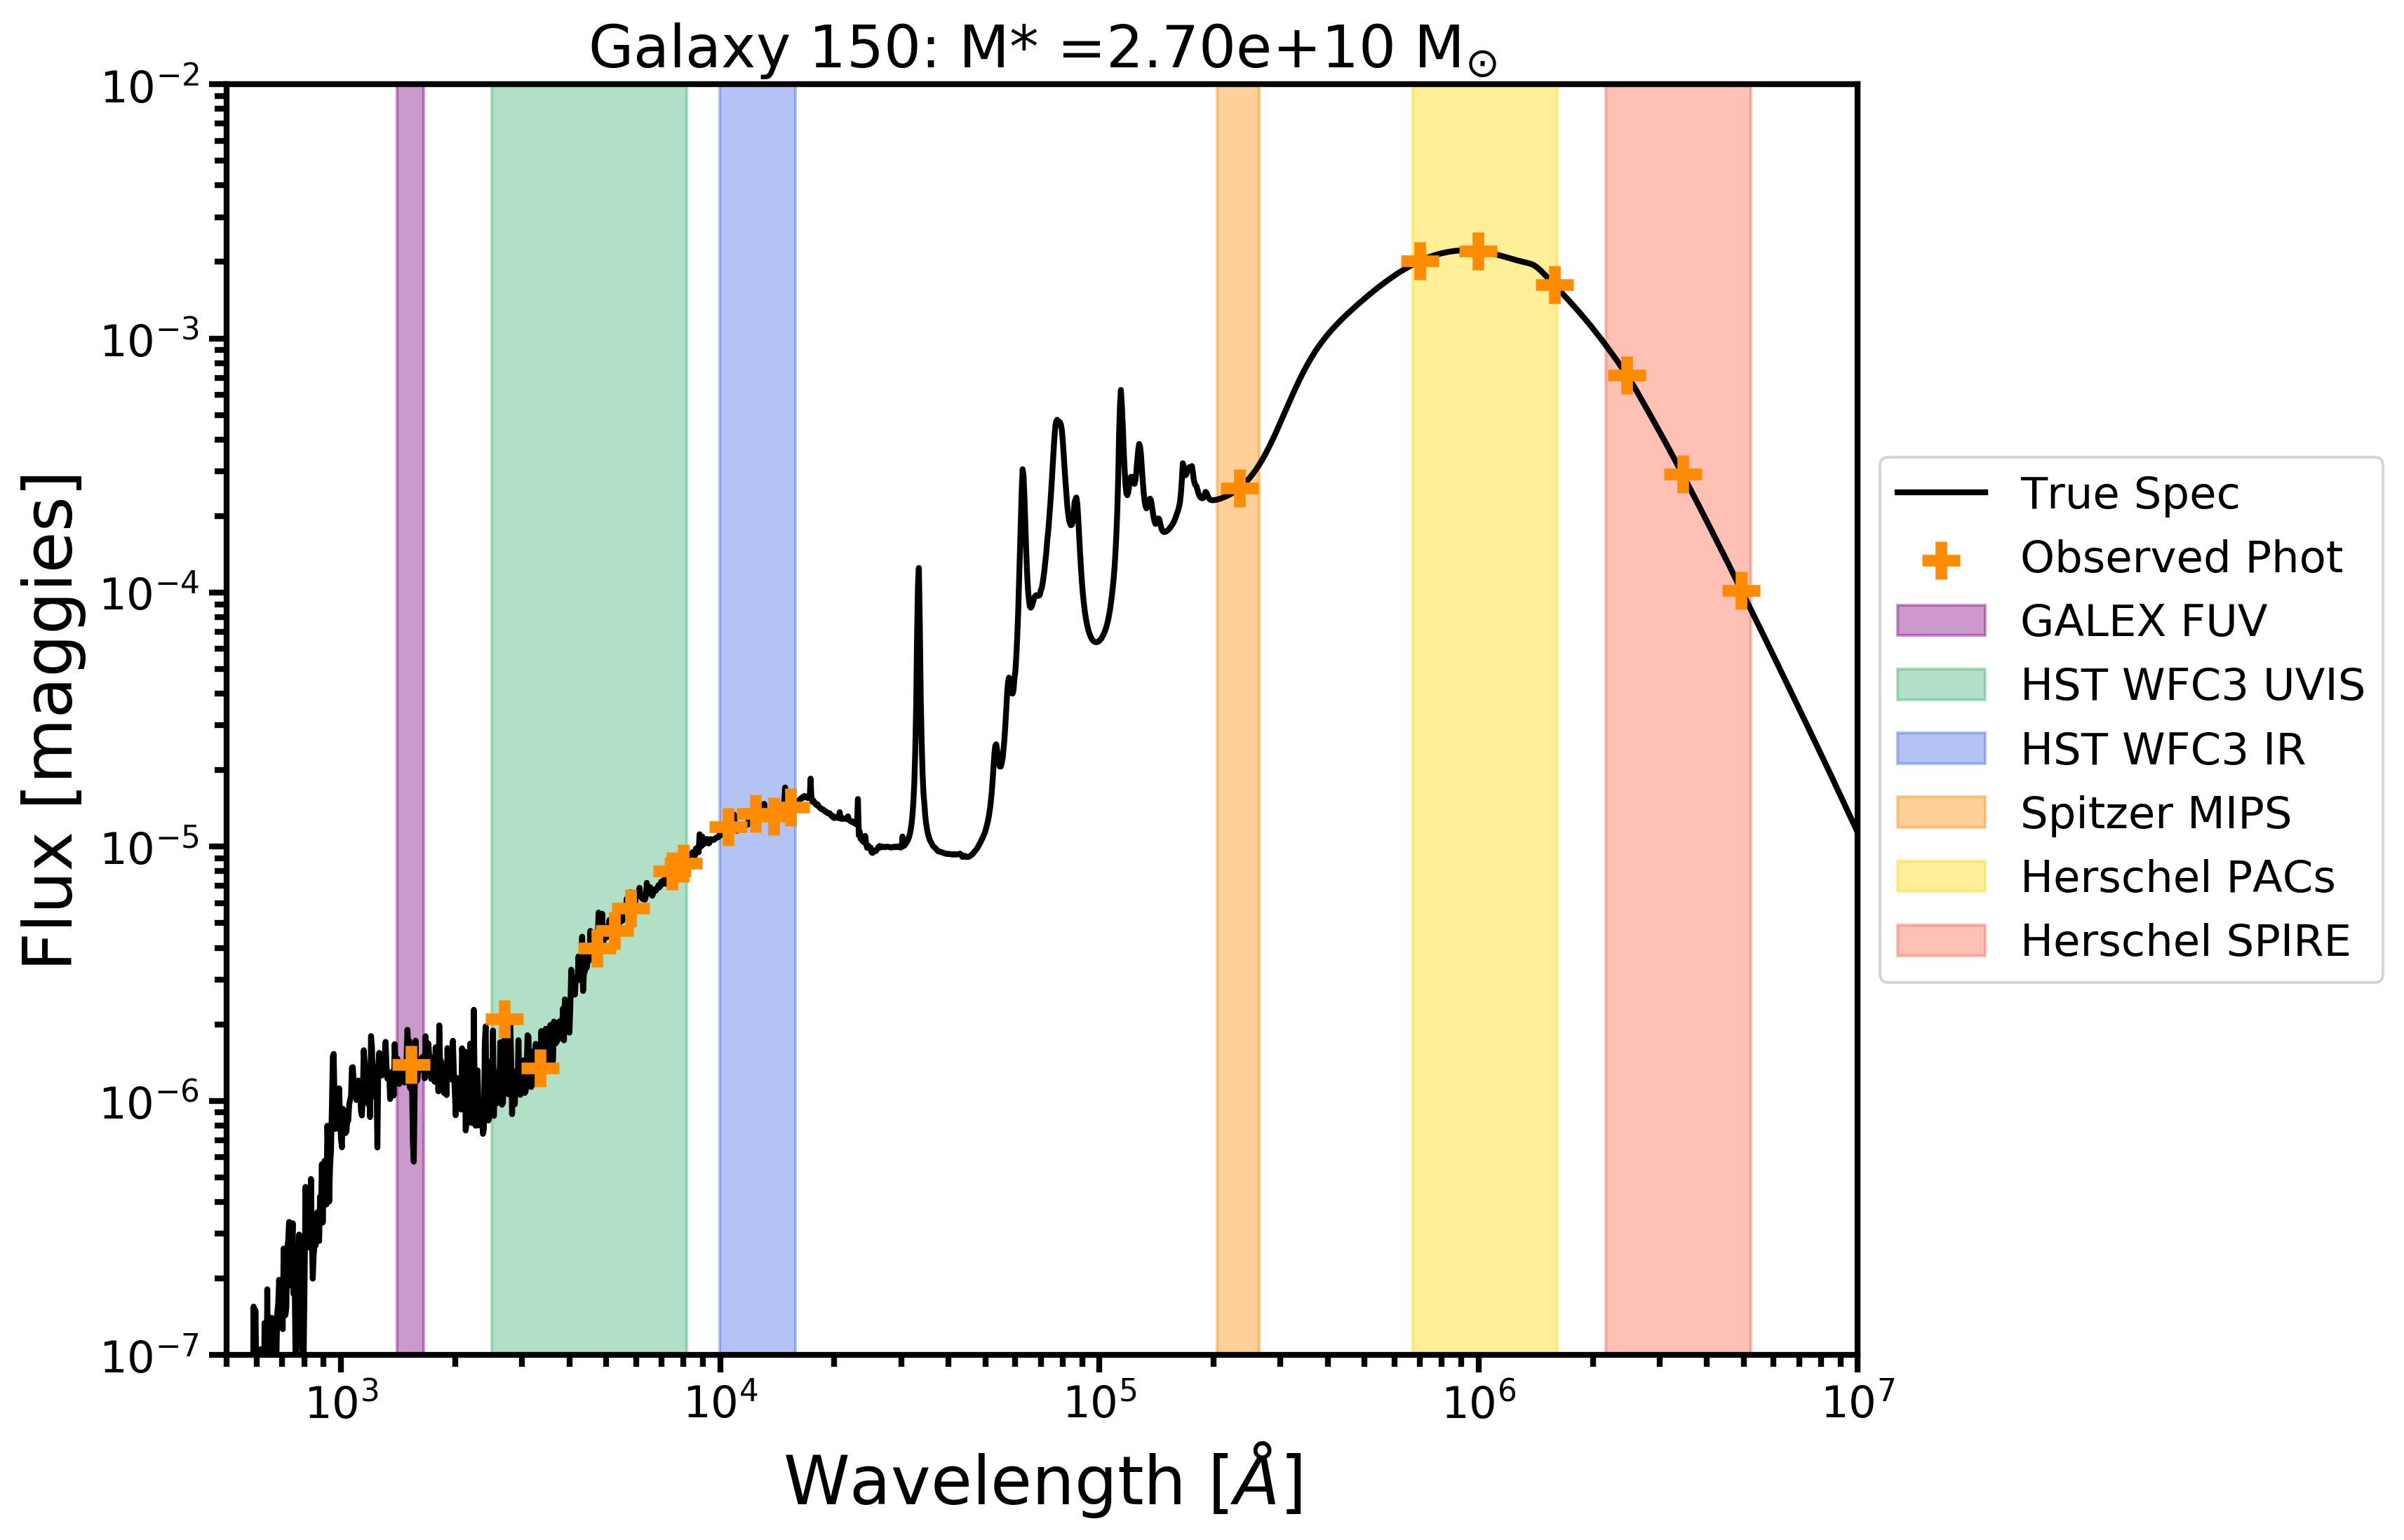
\includegraphics[width = \textwidth]{fancySED_150.png}
    \caption{Example \texttt{powderday} SED with photometric bands highlighted. Each galaxy used fluxes from the same bands with 3\% errors. }
    \label{fig:SED}
\end{figure*}

To assess the validity of various star formation history models, we utilize cosmological simulations to ground-truth the predictions made by each model (stellar mass, mass-weighted age, and star formation rate). We use the \texttt{simba} cosmological simulation, described in full in \cite{dave_simba:_2019}. Briefly, \texttt{simba} is the predecessor of \texttt{mufasa} and relies on \texttt{gizmo}'s meshless finite mass hydrodynamics. New subgrid prescripts for stellar and AGN feedback as well as black hole growth have enabled \texttt{simba} to more accurately reproduce observables like the galaxy stellar mass function and the star forming main sequence. The box size used in our analysis is 25 Mpc h$^{-1}$ with 512$^3$ particles in the entire volume. The minimum resolved mass is 7.3\times 10$^7 \: \mathrm{M}_{\odot}$ while the largest galaxy in the box measures 1.4\times 10$^{12} \: \mathrm{M}_{\odot}$ at redshift zero. We use \texttt{caesar}\footnote{https://bitbucket.org/desika/caesar/src/default/} to identify galaxies in the simulation with a 6D friends-of-friends algorithm (minimum stellar population of a galaxy is set at 32 particles). Around 2500 galaxies are found in the redshift zero snapshot. 

Post-processing radiative transfer is performed on the galaxies with \texttt{powderday}\footnote{https://github.com/dnarayanan/powderday}. \texttt{Powderday} wraps \texttt{FSPS} stellar population synthesis (\cite{conroy_propagation_2009}; \cite{conroy_propagation_2010}) and the \texttt{python} bindings \texttt{python-fsps} and \texttt{hyperion} dust radiative transfer (\cite{robitaille_hyperion:_2011}, resulting in model synthetic SEDs spanning from the UV to submilimeter wavelengths. The additional implementation of a model for the production, growth, and destruction of dust grains in \texttt{simba} (\cite{li_dust--gas_2019}) allows for a more realistic treatment of dust attenuation and emission from galaxies. Individual snapshots were created for each identified galaxy so that contamination from neighboring particles not associated with the selected galaxy was removed. 

We generate mock photometry from the \texttt{powderday} SEDs. We chose photometry at bands corresponding to filters in \texttt{sedpy}\footnote{https://github.com/bd-j/sedpy}, totaling nineteen flux points spanning from the \textit{GALEX FUV} filter at 1542 {\AA} to the \textit{Herschel SPIRE} band at 500 $\mu$m. We fixed uncertainties to 3\% of the flux value, since the aim of this study is not to analyze the affect of photometric uncertainties but rather the systematics that arise from the use of various SFH models. An example SED is seen in Figure \ref{fig:SED}.



\section{SED Fitting}


We use the \texttt{python} code \texttt{prospector}\footnote{https://github.com/bd-j/prospector} (\cite{leja_deriving_2017}; \cite{leja_how_2018}). \texttt{Prospector} derives properties of galaxies by using stellar population synthesis evolved with dust within the framework of \texttt{FSPS}. As both \texttt{powderday} and \texttt{prospector} use \texttt{FSPS} with the same spectral libraries (MILES) and isochrones (MIST) for stellar population synthesis, uncertainties involved with stellar evolution are minimal. (models for AGN and nebular emission are also included in \texttt{Prospector} but were not used with this study as the these components were ignored in the post-processes radiative transfer). \texttt{Prospector} uses a Bayesian framework via \texttt{dynesty} nested sampling (\cite{speagle_dynesty:_2019}) to fit the SEDs and provide posterior distribution estimates of physical parameters such as stellar mass, metallicity, and star formation rate. The power of \texttt{dyensty} lies in its ability to efficiently sample multi-model distributions and have well-defined stopping criteria based evaluations of Bayesian evidence. A key constraint in the model fitting is the concept of energy balance, whereby dust is heated by stars and re-radiates thermally in the FIR, thereby constraining the dust emission to the available energy radiated by stars.


\subsection{Star Formation History}

One of the main components in SED modeling is how to handle stellar evolution. This includes assumptions about initial mass functions, metallicities, stellar evolutionary tracks, and the aggregate star formation history of a galaxy. The effect of the assumed IMF in SED modeling is much debated, but is out of the scope of this analysis as both \texttt{powderday} and \texttt{prospector} assume the same IMF. The focus of this analysis is instead on the impact of the assumed form of the star formation history. As SED modeling codes get more sophisticated, so must the models used in the fitting. As such, non-parametric star formation histories, described not by a functional form but rather by the amount of stellar mass formed in a specific time interval, have become the 'gold standard.' These star formation histories, although less constrained than their parametric counterparts, offer a wider breadth of versatility in terms of reproducing the true star formation history of a galaxy as they are not biased towards a certain shape (i.e. increasing/decreasing star formation over time).  These non-parametric SFHs are informed not by a functional form and the priors for those function parameters, but instead by priors that inform the amount of star formation, and thus stellar mass formed, in a certain time interval. The star formation is constant in each time interval, but the normalization is a free parameter. The difference between the models comes from the priors used to inform this normalization. While parametric models are widely used in the literature, non-parametric models have only just begun to be developed and implemented in next generation SED modeling codes, allowing for greater flexibility in fitting models to observations and an increased accuracy in stellar mass prediction. The non-parametric star formation histories used in this analysis are described in depth in \citep{leja_how_2018}, while I provide a more top level view in the following sections. 




\subsubsection{Parametric Star Formation History}

As a baseline comparison, one parametric star formation history was considered, specifically the delayed tau model, which describes the star formation history of a galaxy as exponentially declining, parameterized by the e-folding time for the SFH that is informed by a log-uniform prior. The free parameters for this model also include the stellar mass formed by the galaxy and the maximum age of the stellar population. Two runs were conducted with this template, one with and one without burst episodes. During a burst, some fraction of mass is formed in an instantaneous burst of star formation. This particular star formation history is a common assumption in SED fitting and thus serves as a comparison to the more sophisticated and flexible non parametric options. An important note is the indirect effects of the priors used for the parameters in this model (tau, age of the galaxy, total stellar mass formed) on the output of the model (observed stellar mass), acting to systematically bias the derived physical parameters and underestimate the uncertainties involved.  


\subsubsection{Dirichlet Star Formation History}


The first non-parametric star formation model is described by a Dirichlet distribution prior on the specific star formation rate in each interval of time. In practice, the fractional mass formed in each time bin is fit for independently of the total mass formed (i.e. the shape of the SFH is separate from the normalization). The marginal probability distribution on each specific star formation rate follows a Dirichlet prior, which is multivariate beta distribution. The time bins can be adjusted in both number and size by the user, but remain fixed during the fit. Where photometric data fails to constrain the star forming history of the galaxy, a constant star formation history is recovered. An additional parameter, called the concentration parameter, is required to fit the SFHs and controls the concentration of stellar mass formation across time bins. Lower concentration values result in more burst-y star formation histories, while higher values result in smoother SFHs. A value of 0.7 was used for these fits, allowing for moderate bursts of star formation after tests with values of 0.2 and 1.0 failed to match the true star formation histories in a majority of galaxies. This point is explored further in section 4.2. 


\begin{figure}[h]

\centering
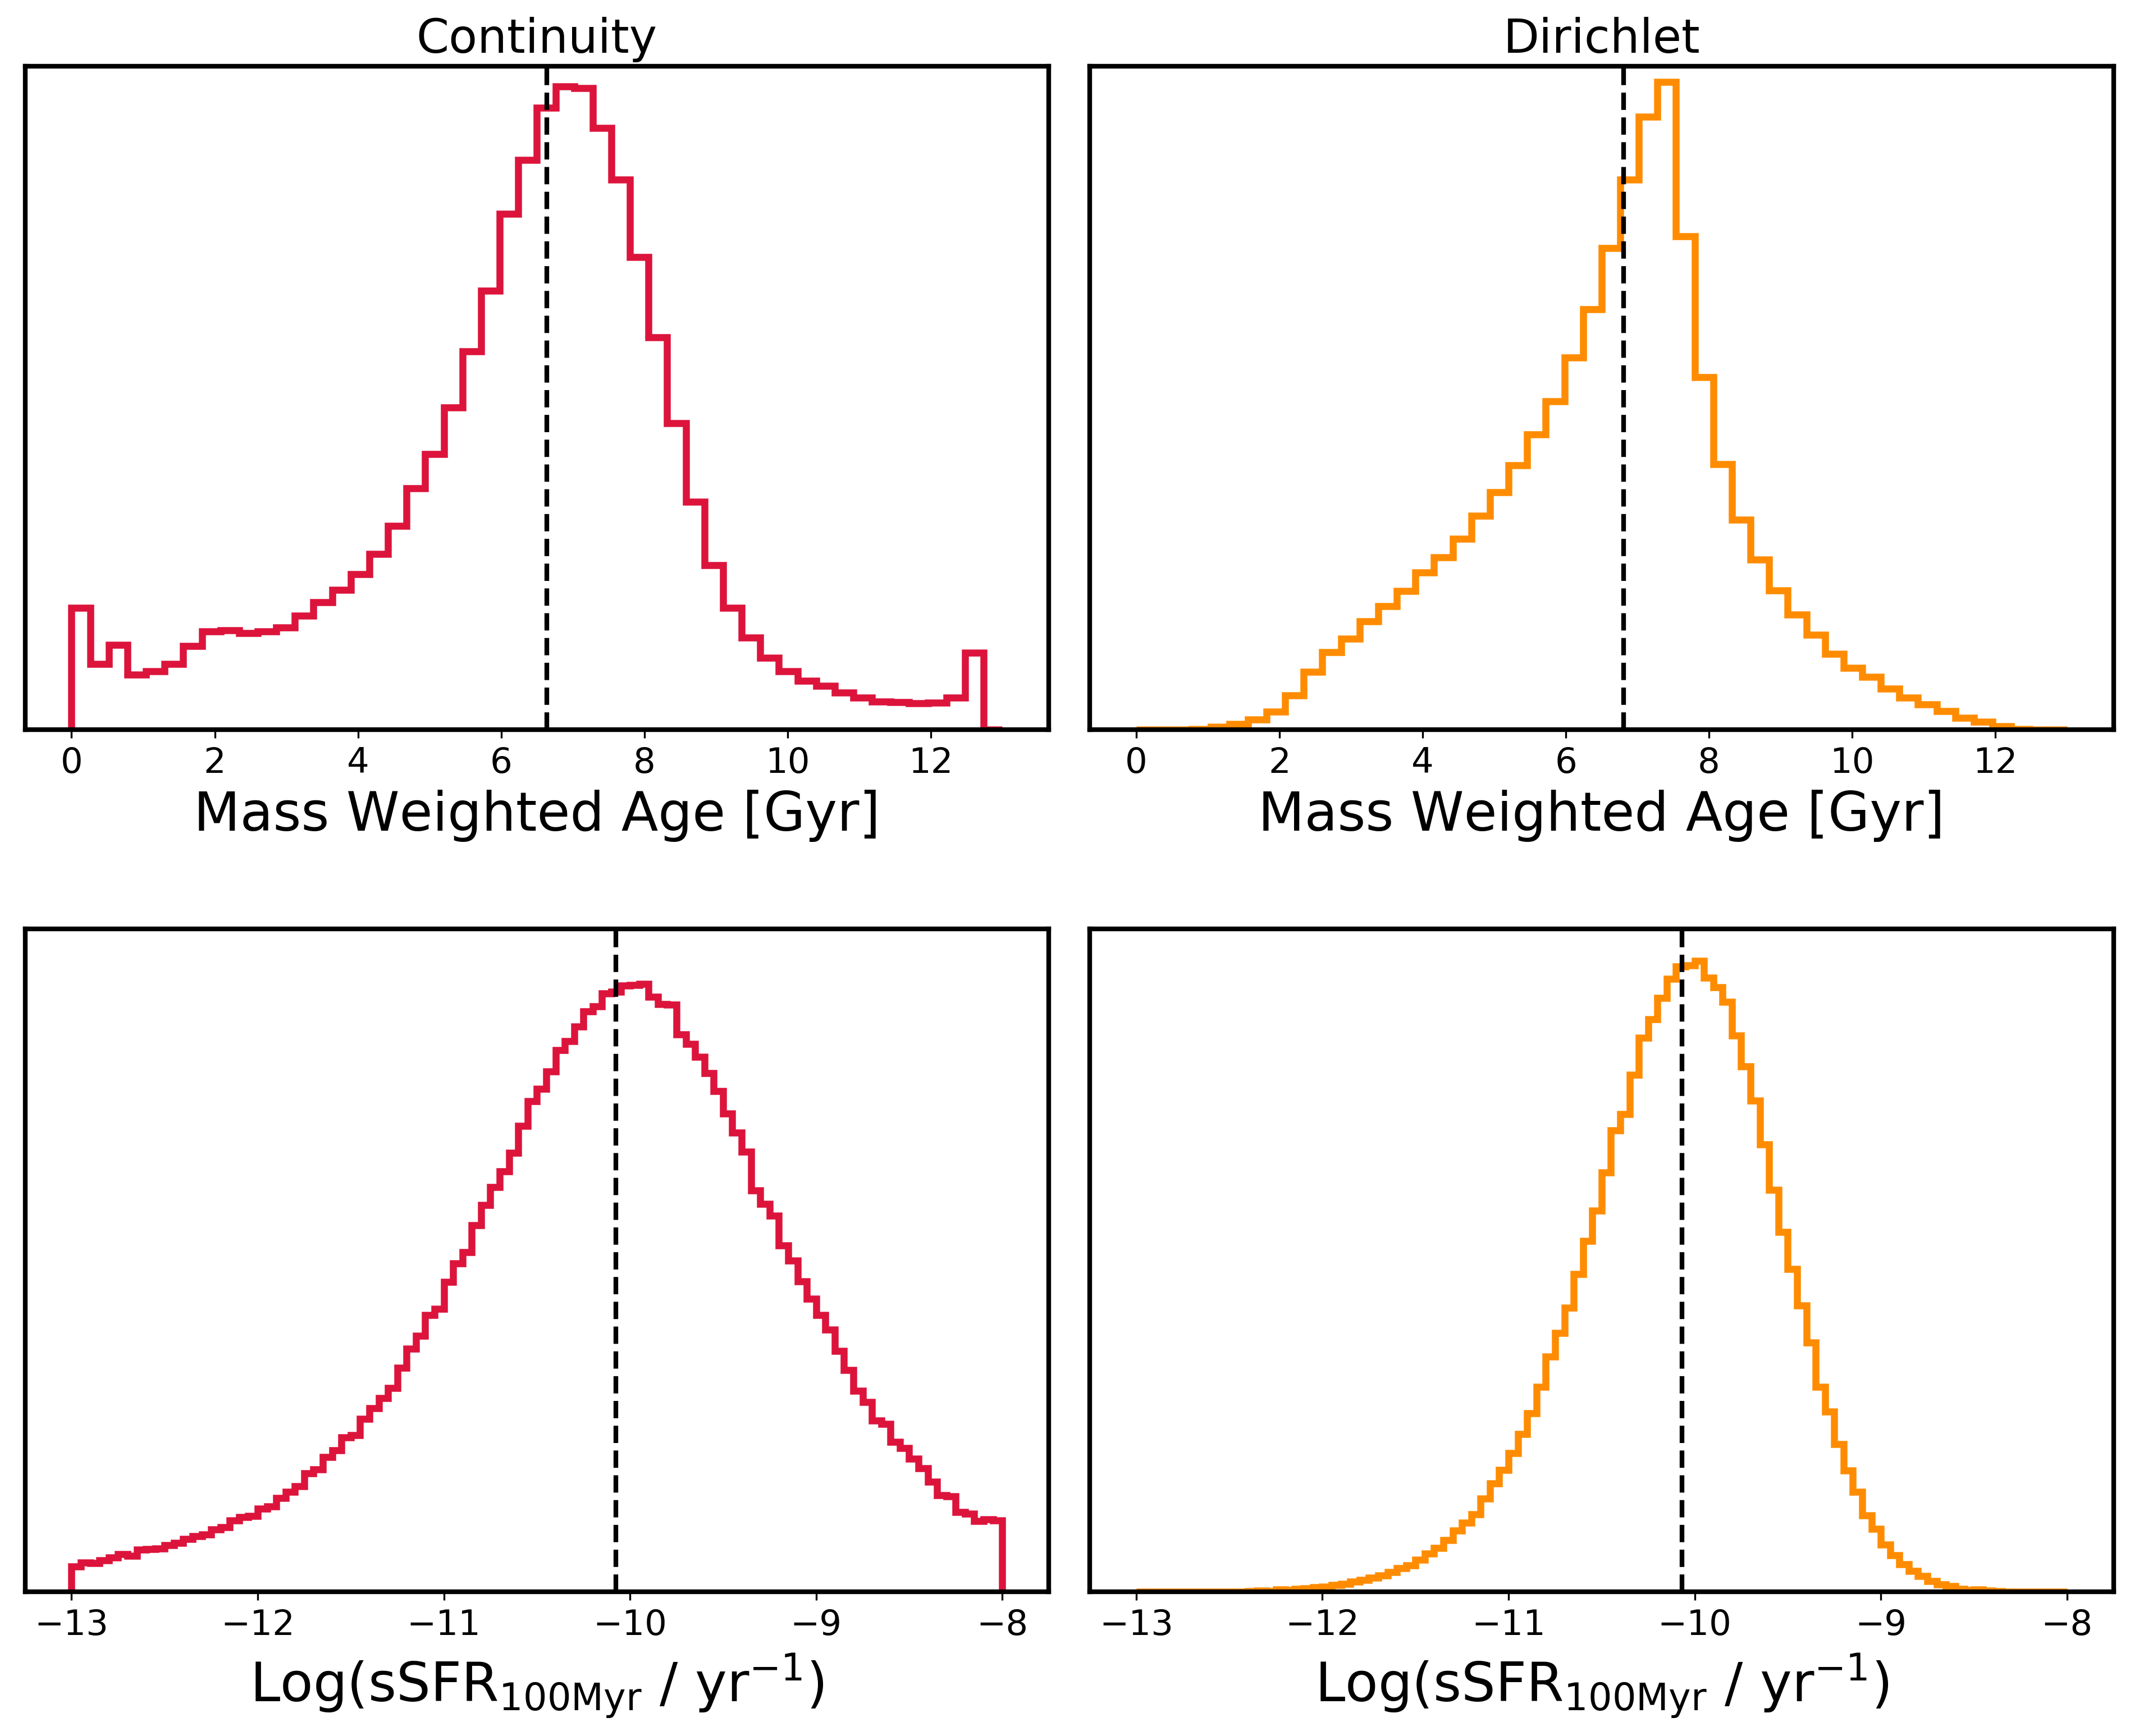
\includegraphics[width=0.5\textwidth]{nonpara_priors.png}\hfill

\caption{Prior distributions for star formation rate and mass-weighted age from the non-parametric star formation history priors.}
\label{fig:priors}

\end{figure}

\subsubsection{Continuity Star Formation History}

The continuity star formation history models the SFH as constant in certain time intervals (number and size adjustable by the user) with normalization informed by a continuity prior, such that sharp changes in the star formation rate across time intervals are weighted against. The continuity prior, described by the Student's - t distribution, informs the difference in adjacent star formation rates ($\mathrm{log}(SFR_n / SFR_{n+1})$). As seen in Figure \ref{fig:priors}, the continuity prior allows for both a minimally and maximally old stellar population. Additionally, both non-parametric SFH priors impose a prior directly on the recent specific star formation history of a galaxy, such that the median of the prior distribution on $\mathrm{log}(sSFR_{100 \: \mathrm{Myr}})$ is roughly $\mathrm{log}(1 / t_{\mathrm{univ}}) \sim -10.1 \: \mathrm{yr}^{-1}$, but the benefit of the continuity prior is that this median can be controlled directly through the mean of the Student's - t distribution.  



\subsection{Metallicity and Dust}

We use the same metallicity and dust models regardless of star formation history model. This allows for isolation of SFH model uncertainty. 

\textbf{Metallicity}: Following \cite{leja_older_2019}, we use a prior on the stellar metallicities as a modified version of the stellar mass–stellar metallicity relationship from z = 0 Sloan Digital Sky Survey (SDSS) data (\cite{gallazzi_ages_2005}). 

\textbf{Dust Attenuation}: We use a modified Calzetti attenuation curve (\cite{calzetti_dust_2001}) to describe the attenuation of stellar light by dust. This model includes variable optical depth towards younger and older stellar populations, a power-law slope, and a variable UV bump strength at 2175 {\AA}. This parameterization is most similar to the model described in \cite{noll_analysis_2009}.   

\textbf{Dust Emission}: Constrained by energy balance, dust emission is described modeled following \cite{draine_infrared_2007}, which describes dust emission using three parameters: U$_{min}$ which is the the minimum radiation field strength in units of the MW value, q$_{PAH}$ which is the mass fraction of dust in PAH form, and $\Gamma$ which is the fraction of dust in high radiation fields. As with the dust attenuation, all parameters are free and have the same prior distributions in all star formation history runs. 



\section{Results} 

We fit SEDs for all SFH models described above. The following sections detail the results of the output of each SED fit, including stellar masses in section 4.1, star formation histories in section 4.2, and star formation rates and stellar ages in section 4.3. 

\subsection{Stellar Mass}

The primary objective of our analysis was recovering the stellar masses and understanding the underlying uncertainties in the fits. Figure \ref{fig:mass_comp} shows the results the stellar mass estimates, comparing the derived stellar masses from the various star formation history models to the true stellar mass values. The stellar masses estimated from the two non-parametric models show good agreement with the true stellar masses -- for the Dirichlet prior, to less than 0.5 dex for a majority of galaxies. 

\begin{figure*}[h]
    \centering
    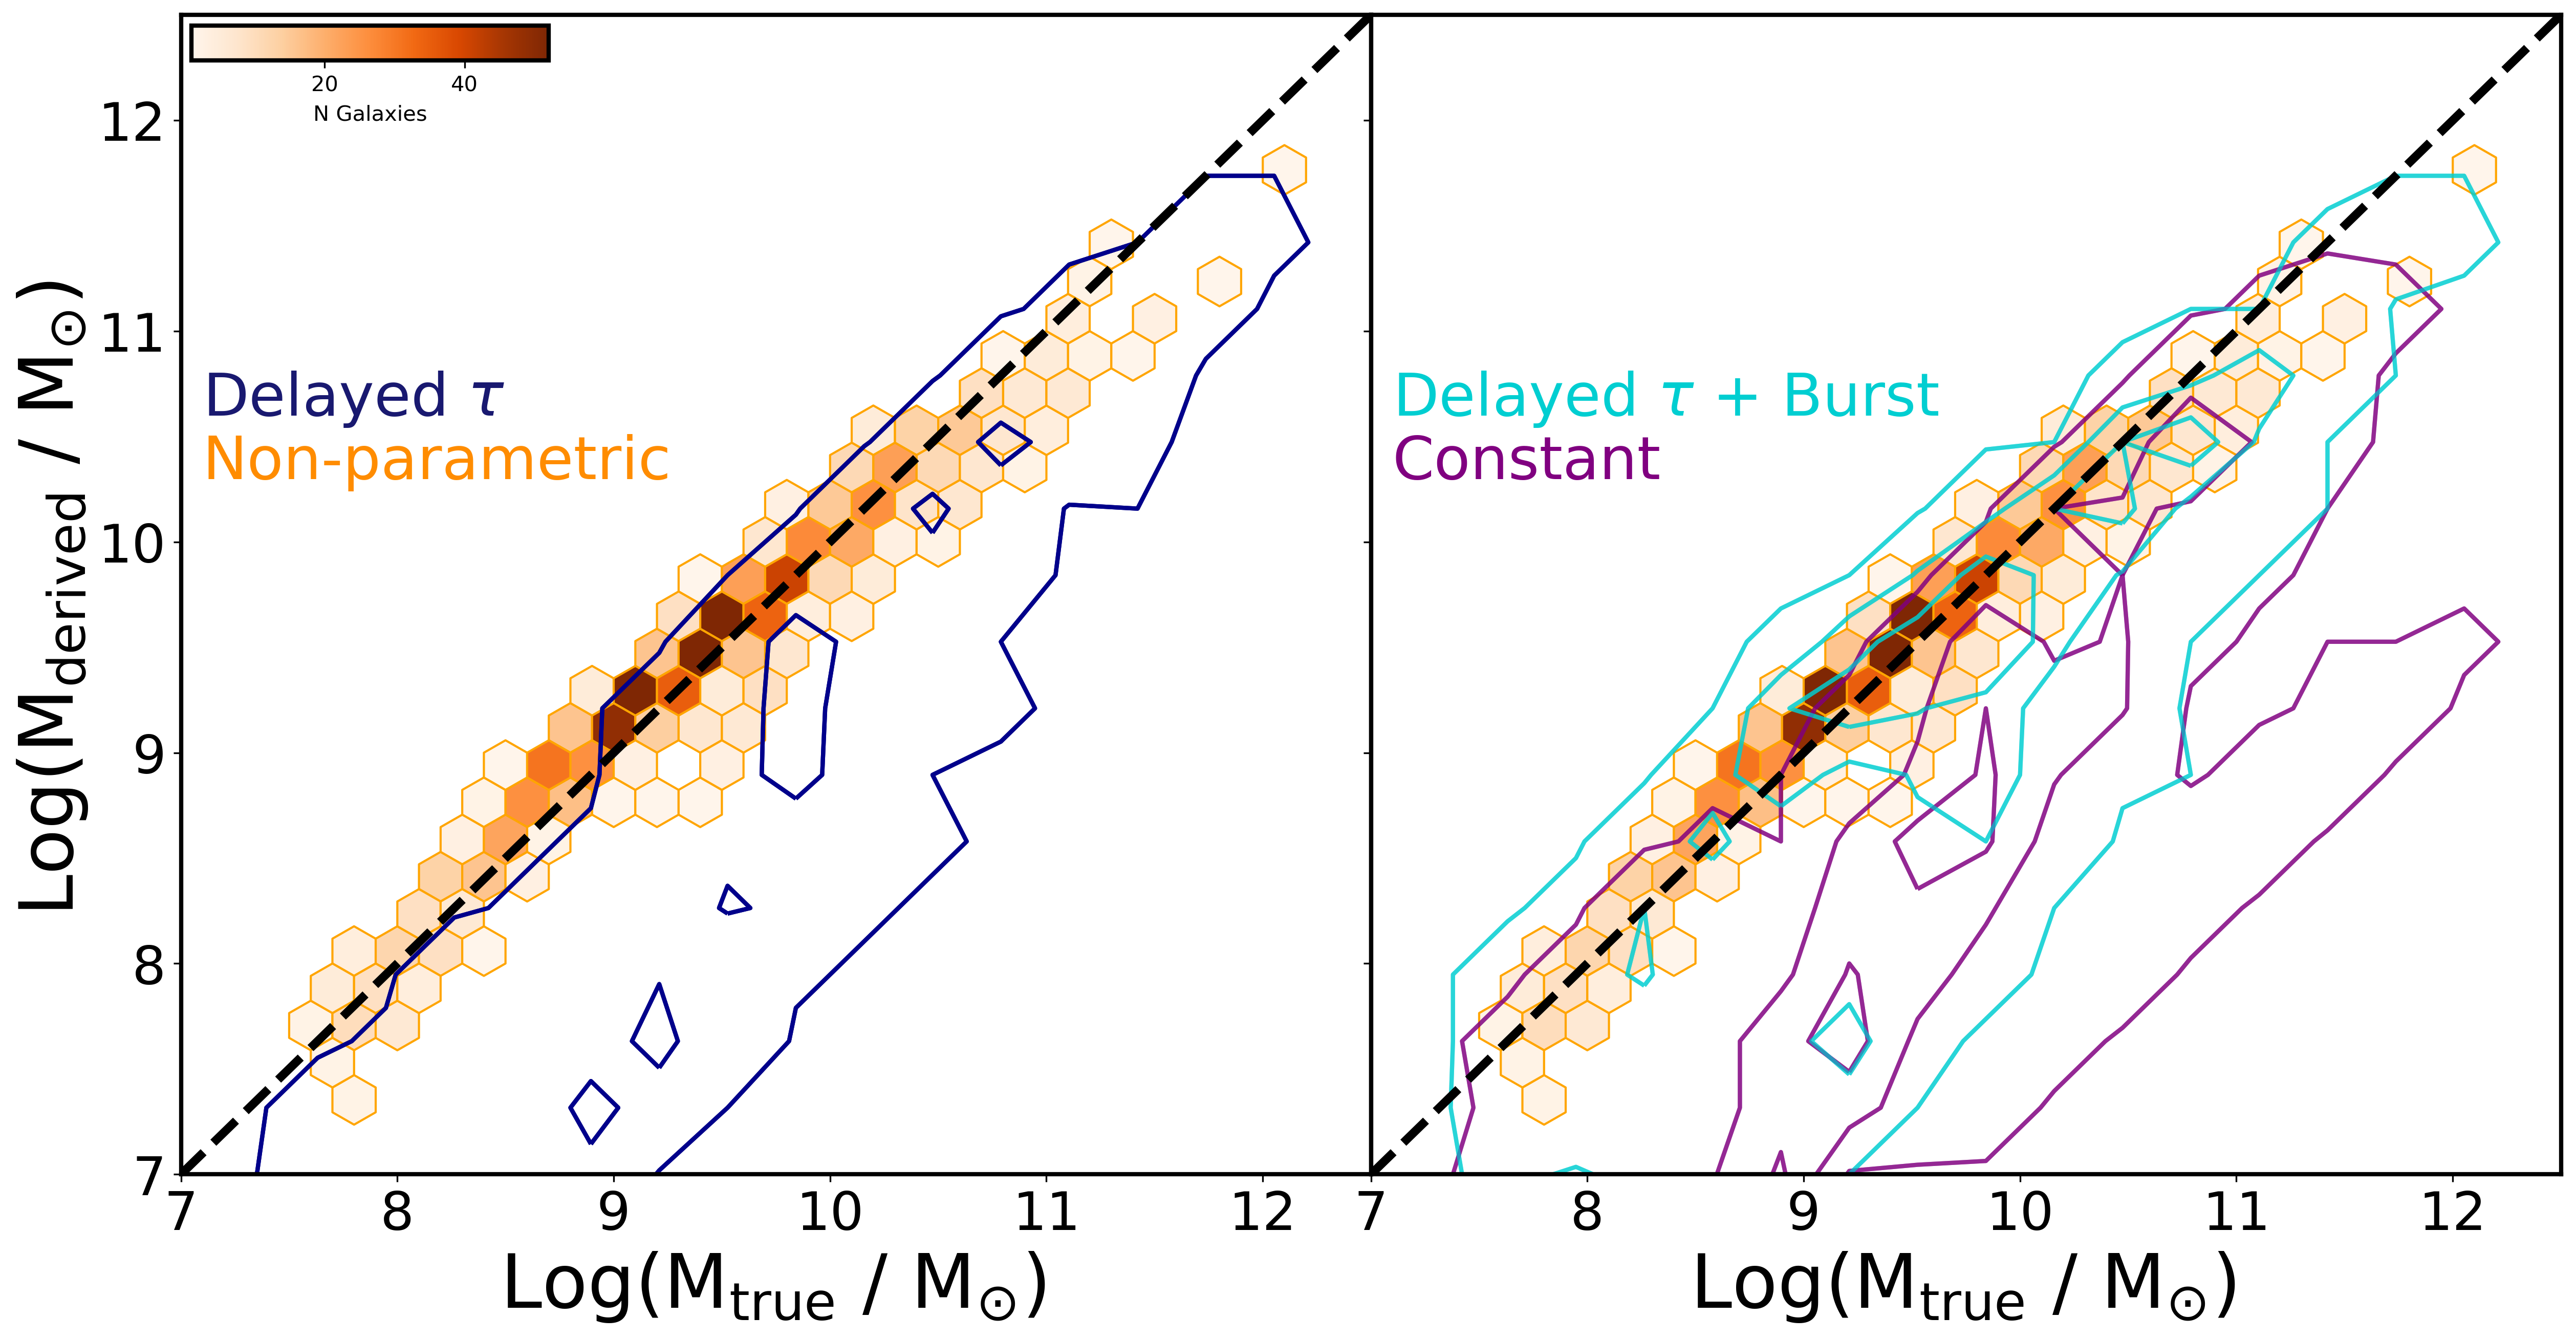
\includegraphics[width=\textwidth]{mass_comp.png}\hfill
    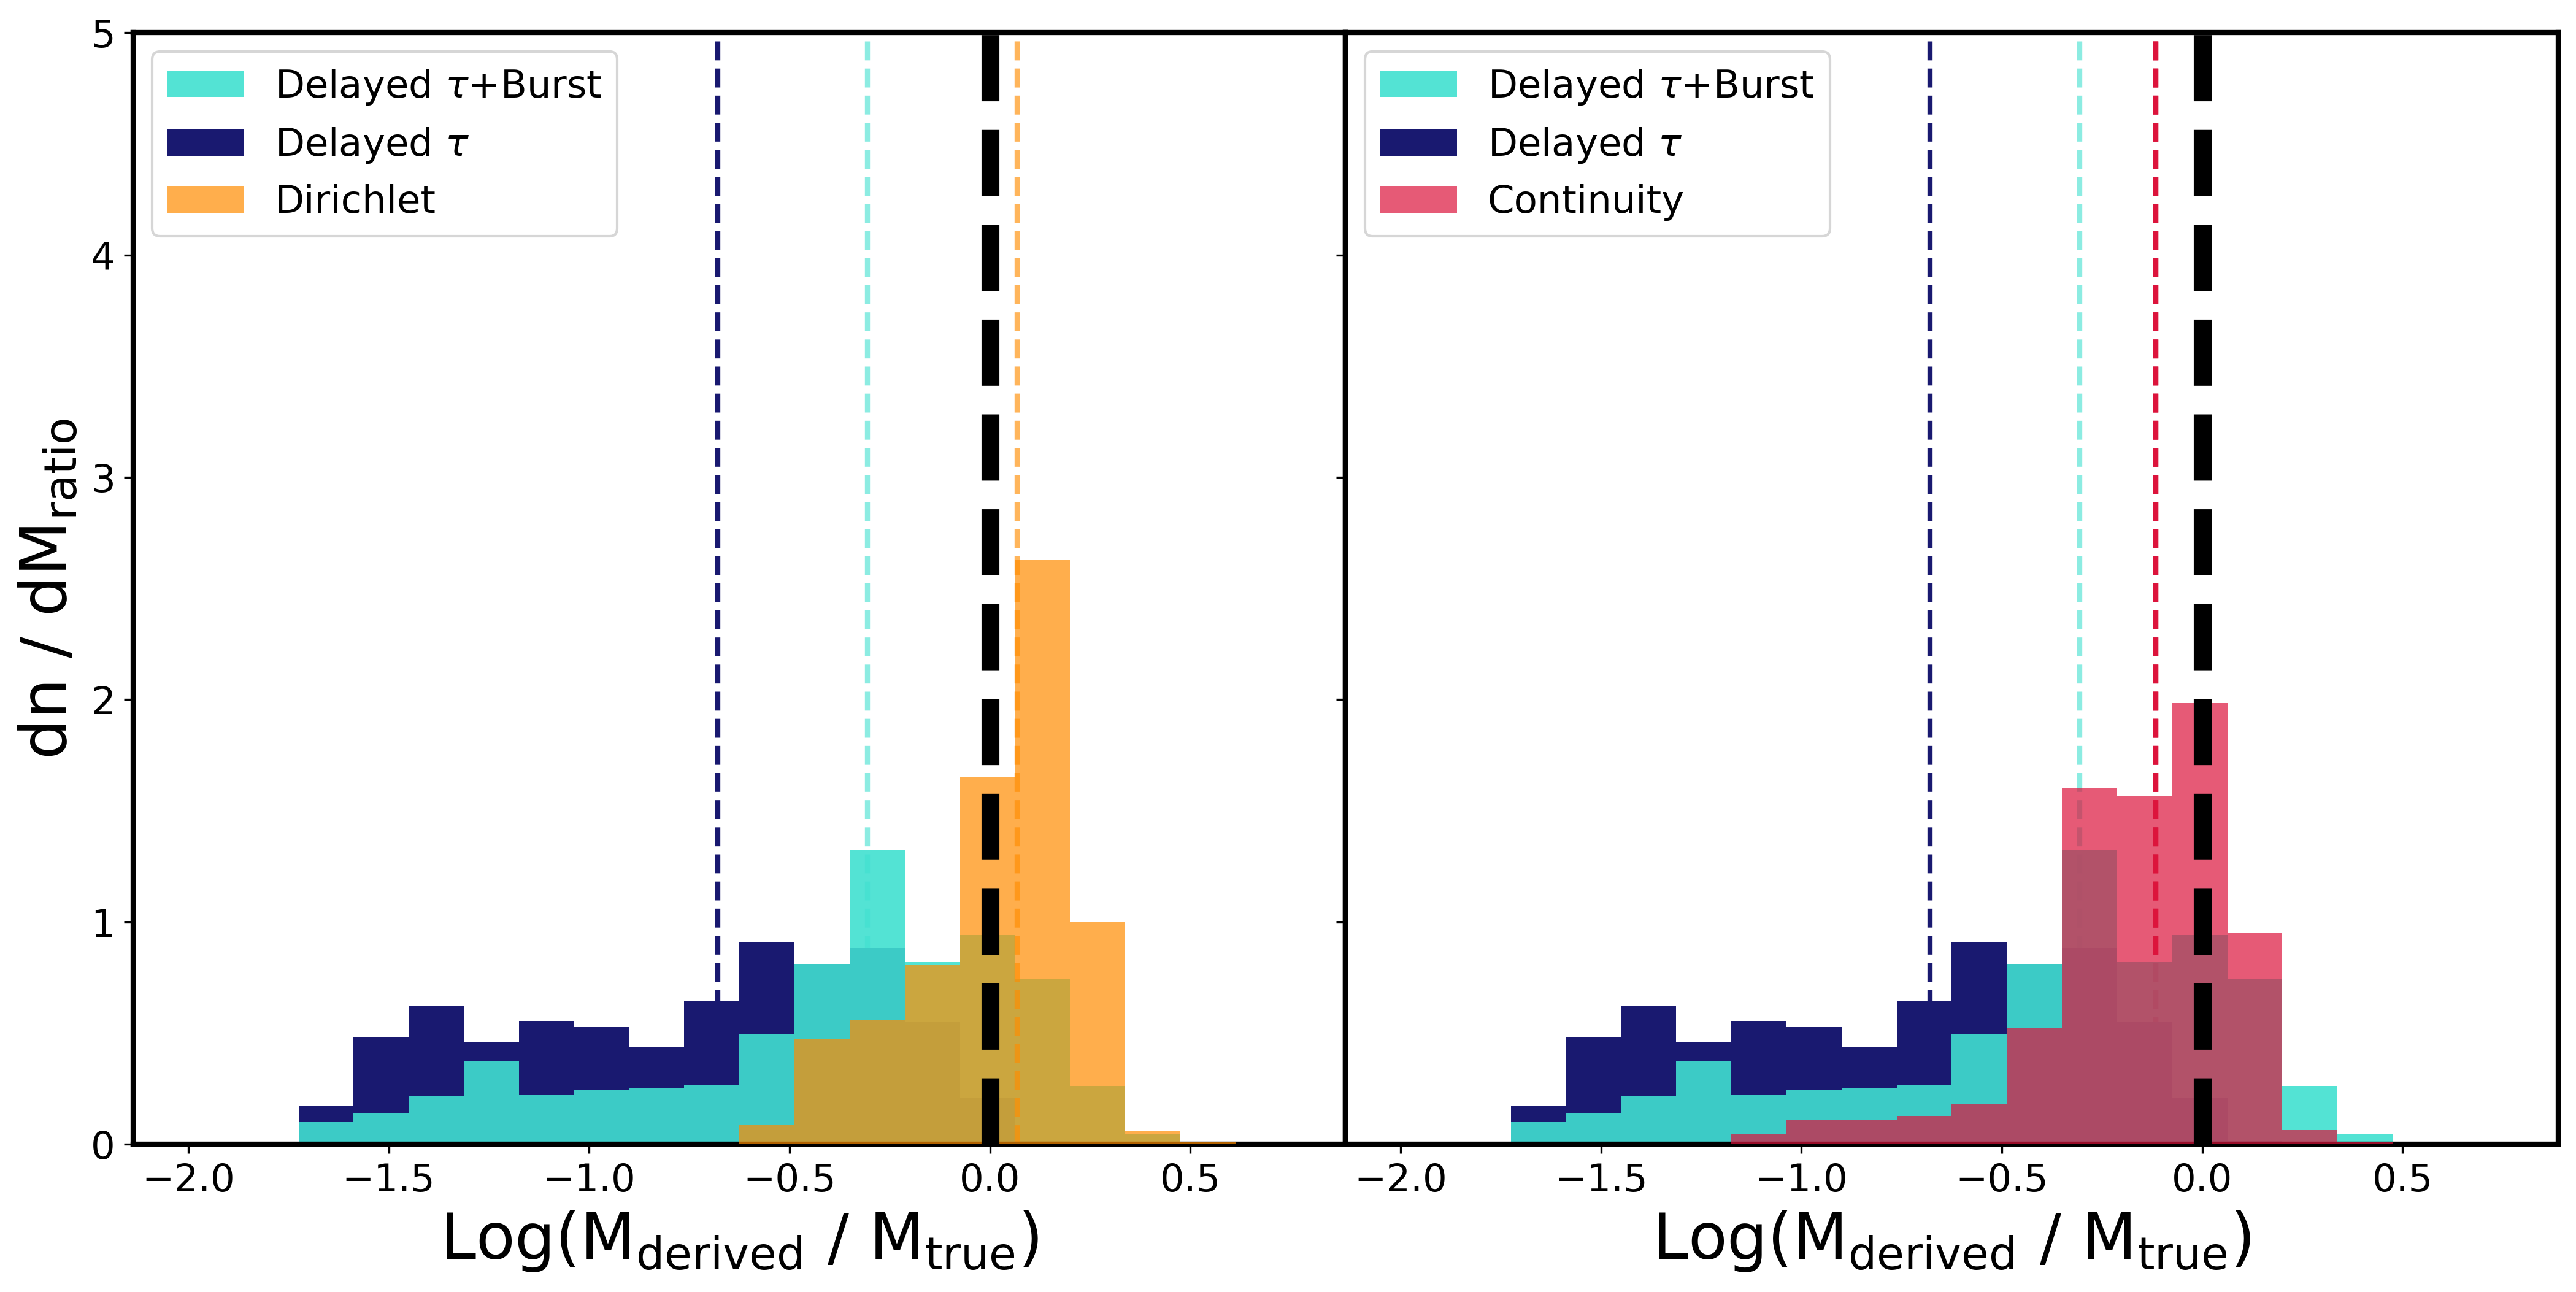
\includegraphics[width=\textwidth]{ratio_hist_ultra.png}\hfill
    
    \caption{Top: Comparison of derived stellar masses to the true stellar mass. Left in orange hexes are masses derived from the Dirichlet prior. Right in red hexes are masses derived from the Continuity prior. The masses derived from the parametric SFHs are in dark blue and turquoise. Bottom: Distribution of estimated to true stellar mass ratios. Medians of the distributions are shown with the dotted lines.}
    \label{fig:mass_comp}
\end{figure*}

As compared to the parametric star formation histories, both the median of the estimated stellar mass distribution and the scatter are improved with the non-parametric SFHs. 

\subsection{Star Formation History Recovery}

A critical step in recovering the true stellar mass is to properly estimate the shape of the star formation history. That the non-parametric star formation histories are more accurate at recovering the stellar mass of a galaxy is mainly attributed to the fact that they are much more flexible and thus better at describing the various star formation histories seen with the \texttt{simba} galaxies. With only a small number of parameters describing the width and location of the curve, the two parametric SFHs (delayed $\tau$ and delayed $\tau$ with a burst component), struggle to match the true SFH for most galaxies. This will affect not only the estimated stellar mass but also the stellar ages. 

\begin{figure}[h]

\centering
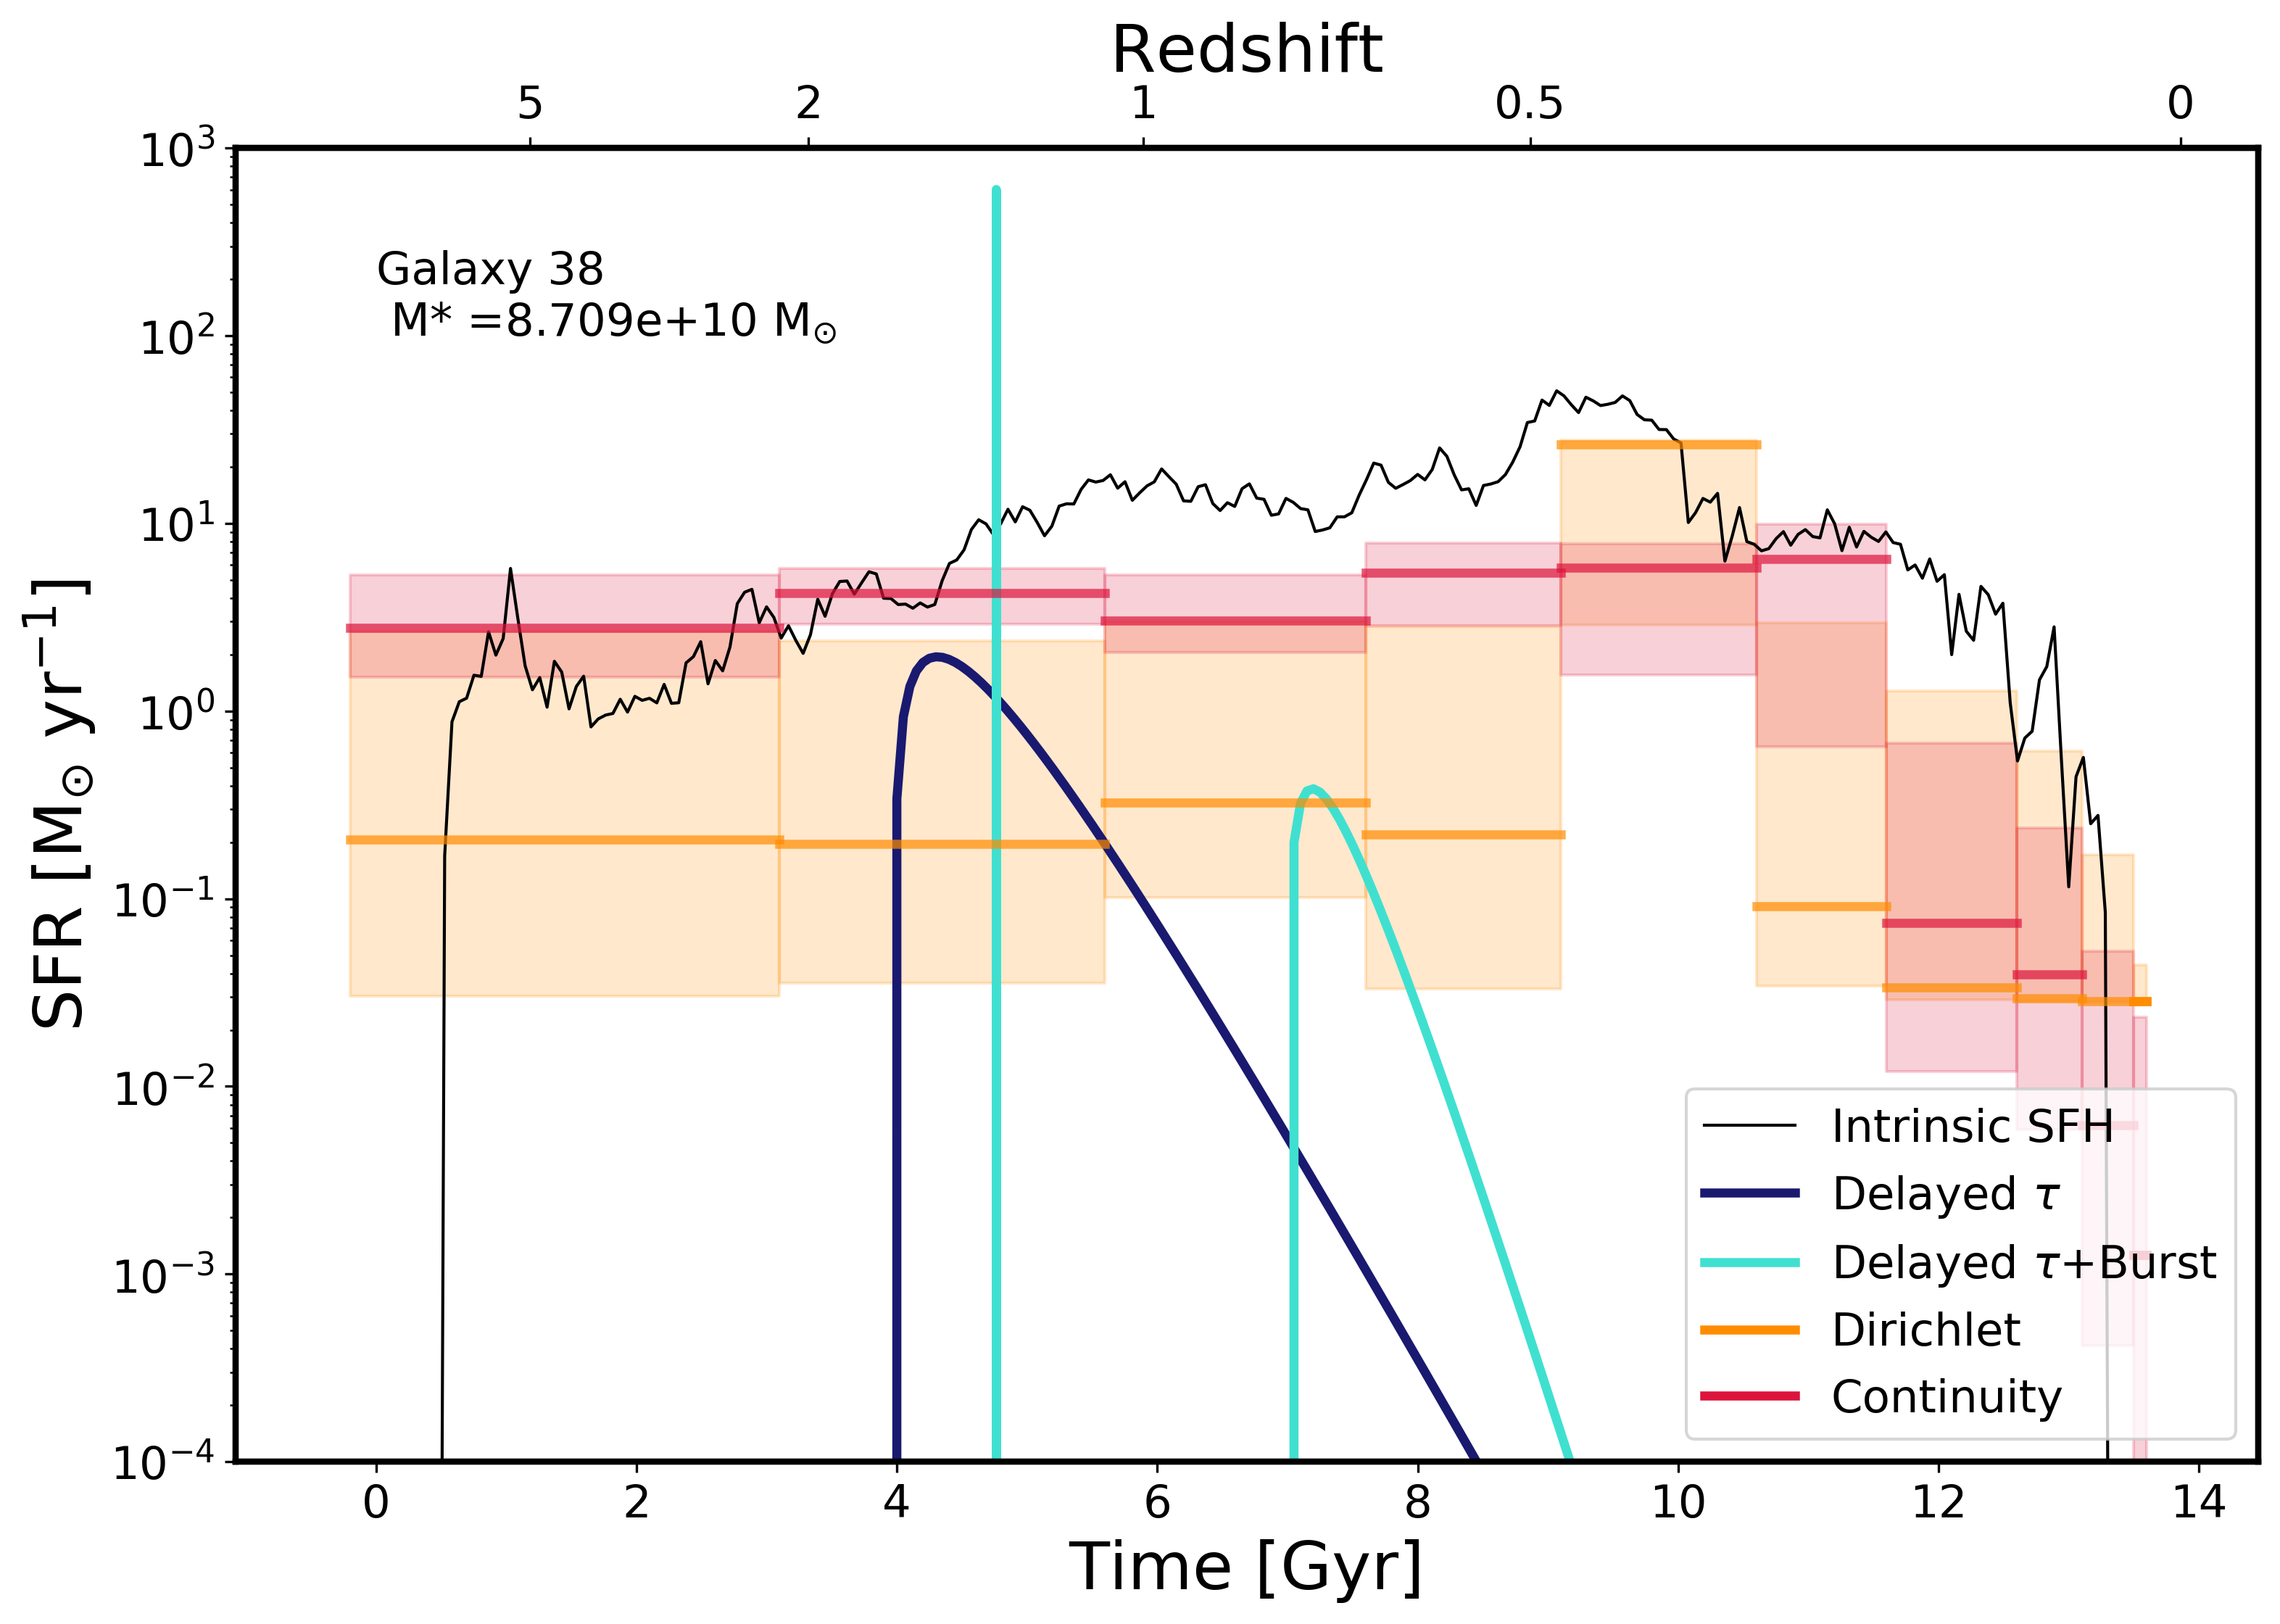
\includegraphics[width=0.47\textwidth]{SFH_38.png}

\caption{Star formation history for an example galaxy. The 50$^{\mathrm{th}}$ percentile value is shown as the solid line for the non-parametric SFHs while the shaded regions include the 16$^{\mathrm{th}}$ through 84$^{\mathrm{th}}$ percentiles.}
\label{fig:sfh}

\end{figure}



\subsection{Ages and Star Formation Rates}

We can also take a look at the estimated star formation rates and mass-weighted stellar ages. Both properties provide further diagnostics into the power of non-parametric star formation histories, as recovering the true star formation history of a galaxy requires estimating both the stellar mass and age of the stars formed. As seen in Figure \ref{fig:age_sfr}, the non-parametric SFHs systematically overestimate the late time star formation rate of galaxies. On the other hand, the stellar ages are, even with considerable scatter, accurate on average. The cause of the overestimation seen in SFR$_{100 \: \mathrm{Myr}}$ is discussed in Section 5.2, where we explore various origins of the discrepancies in stellar mass estimates.

\begin{figure}[h]

\centering
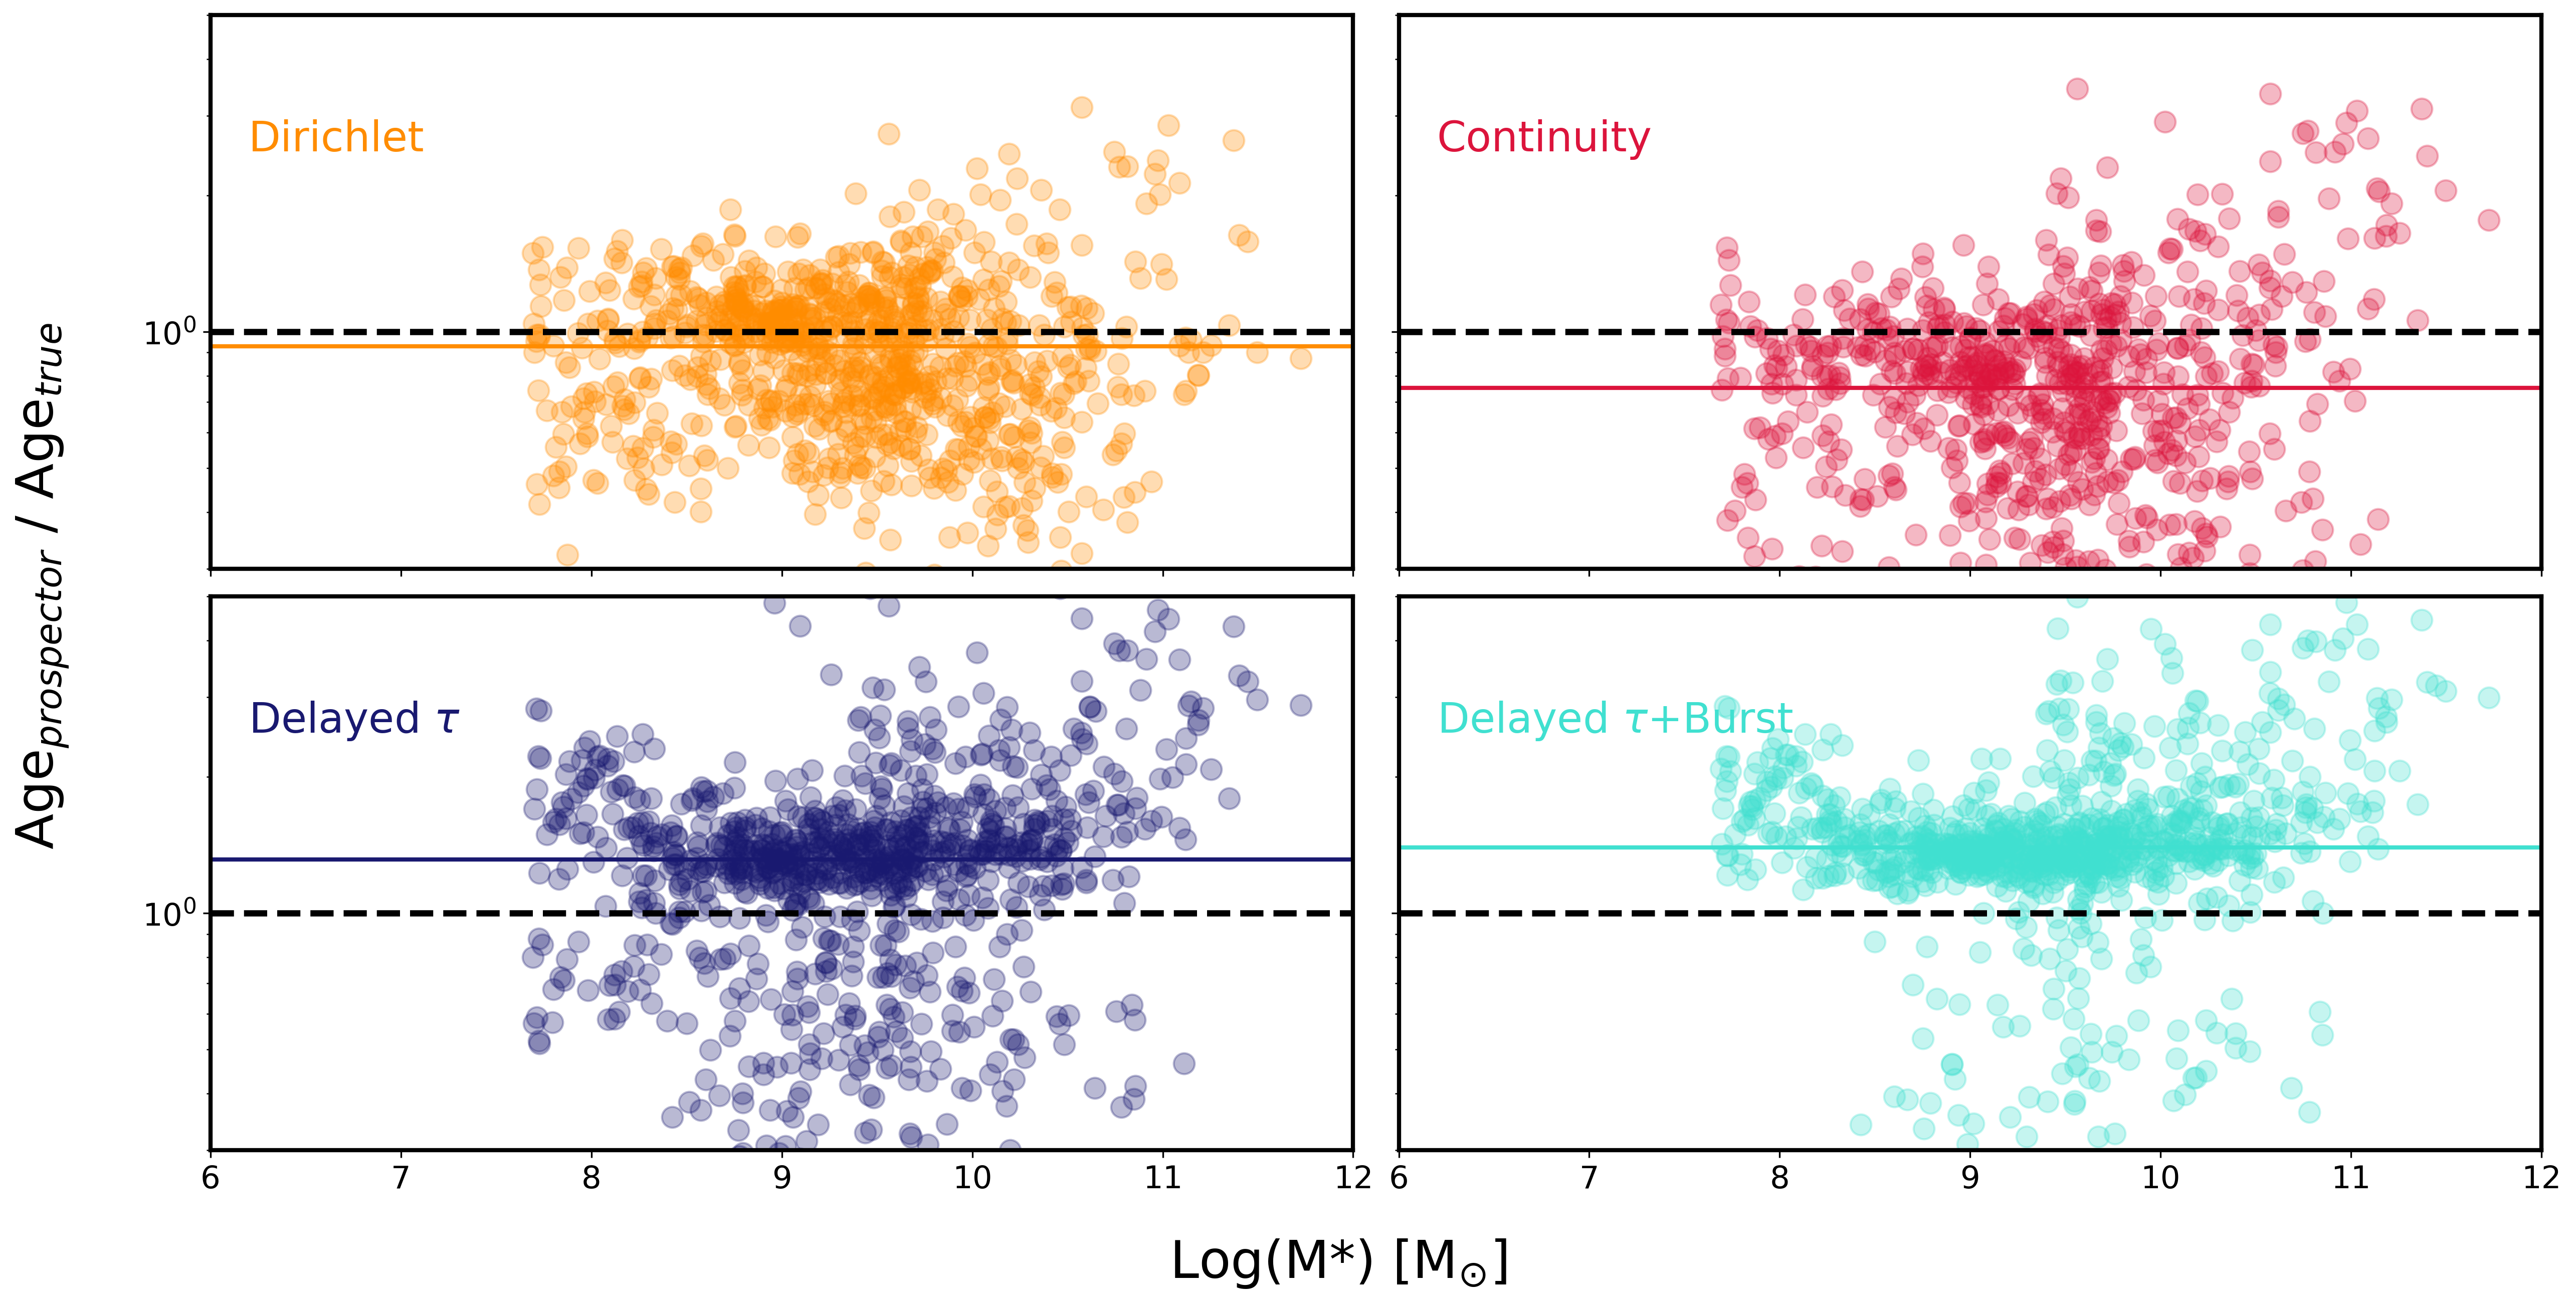
\includegraphics[width=0.5\textwidth]{ages_comp.png}\hfill
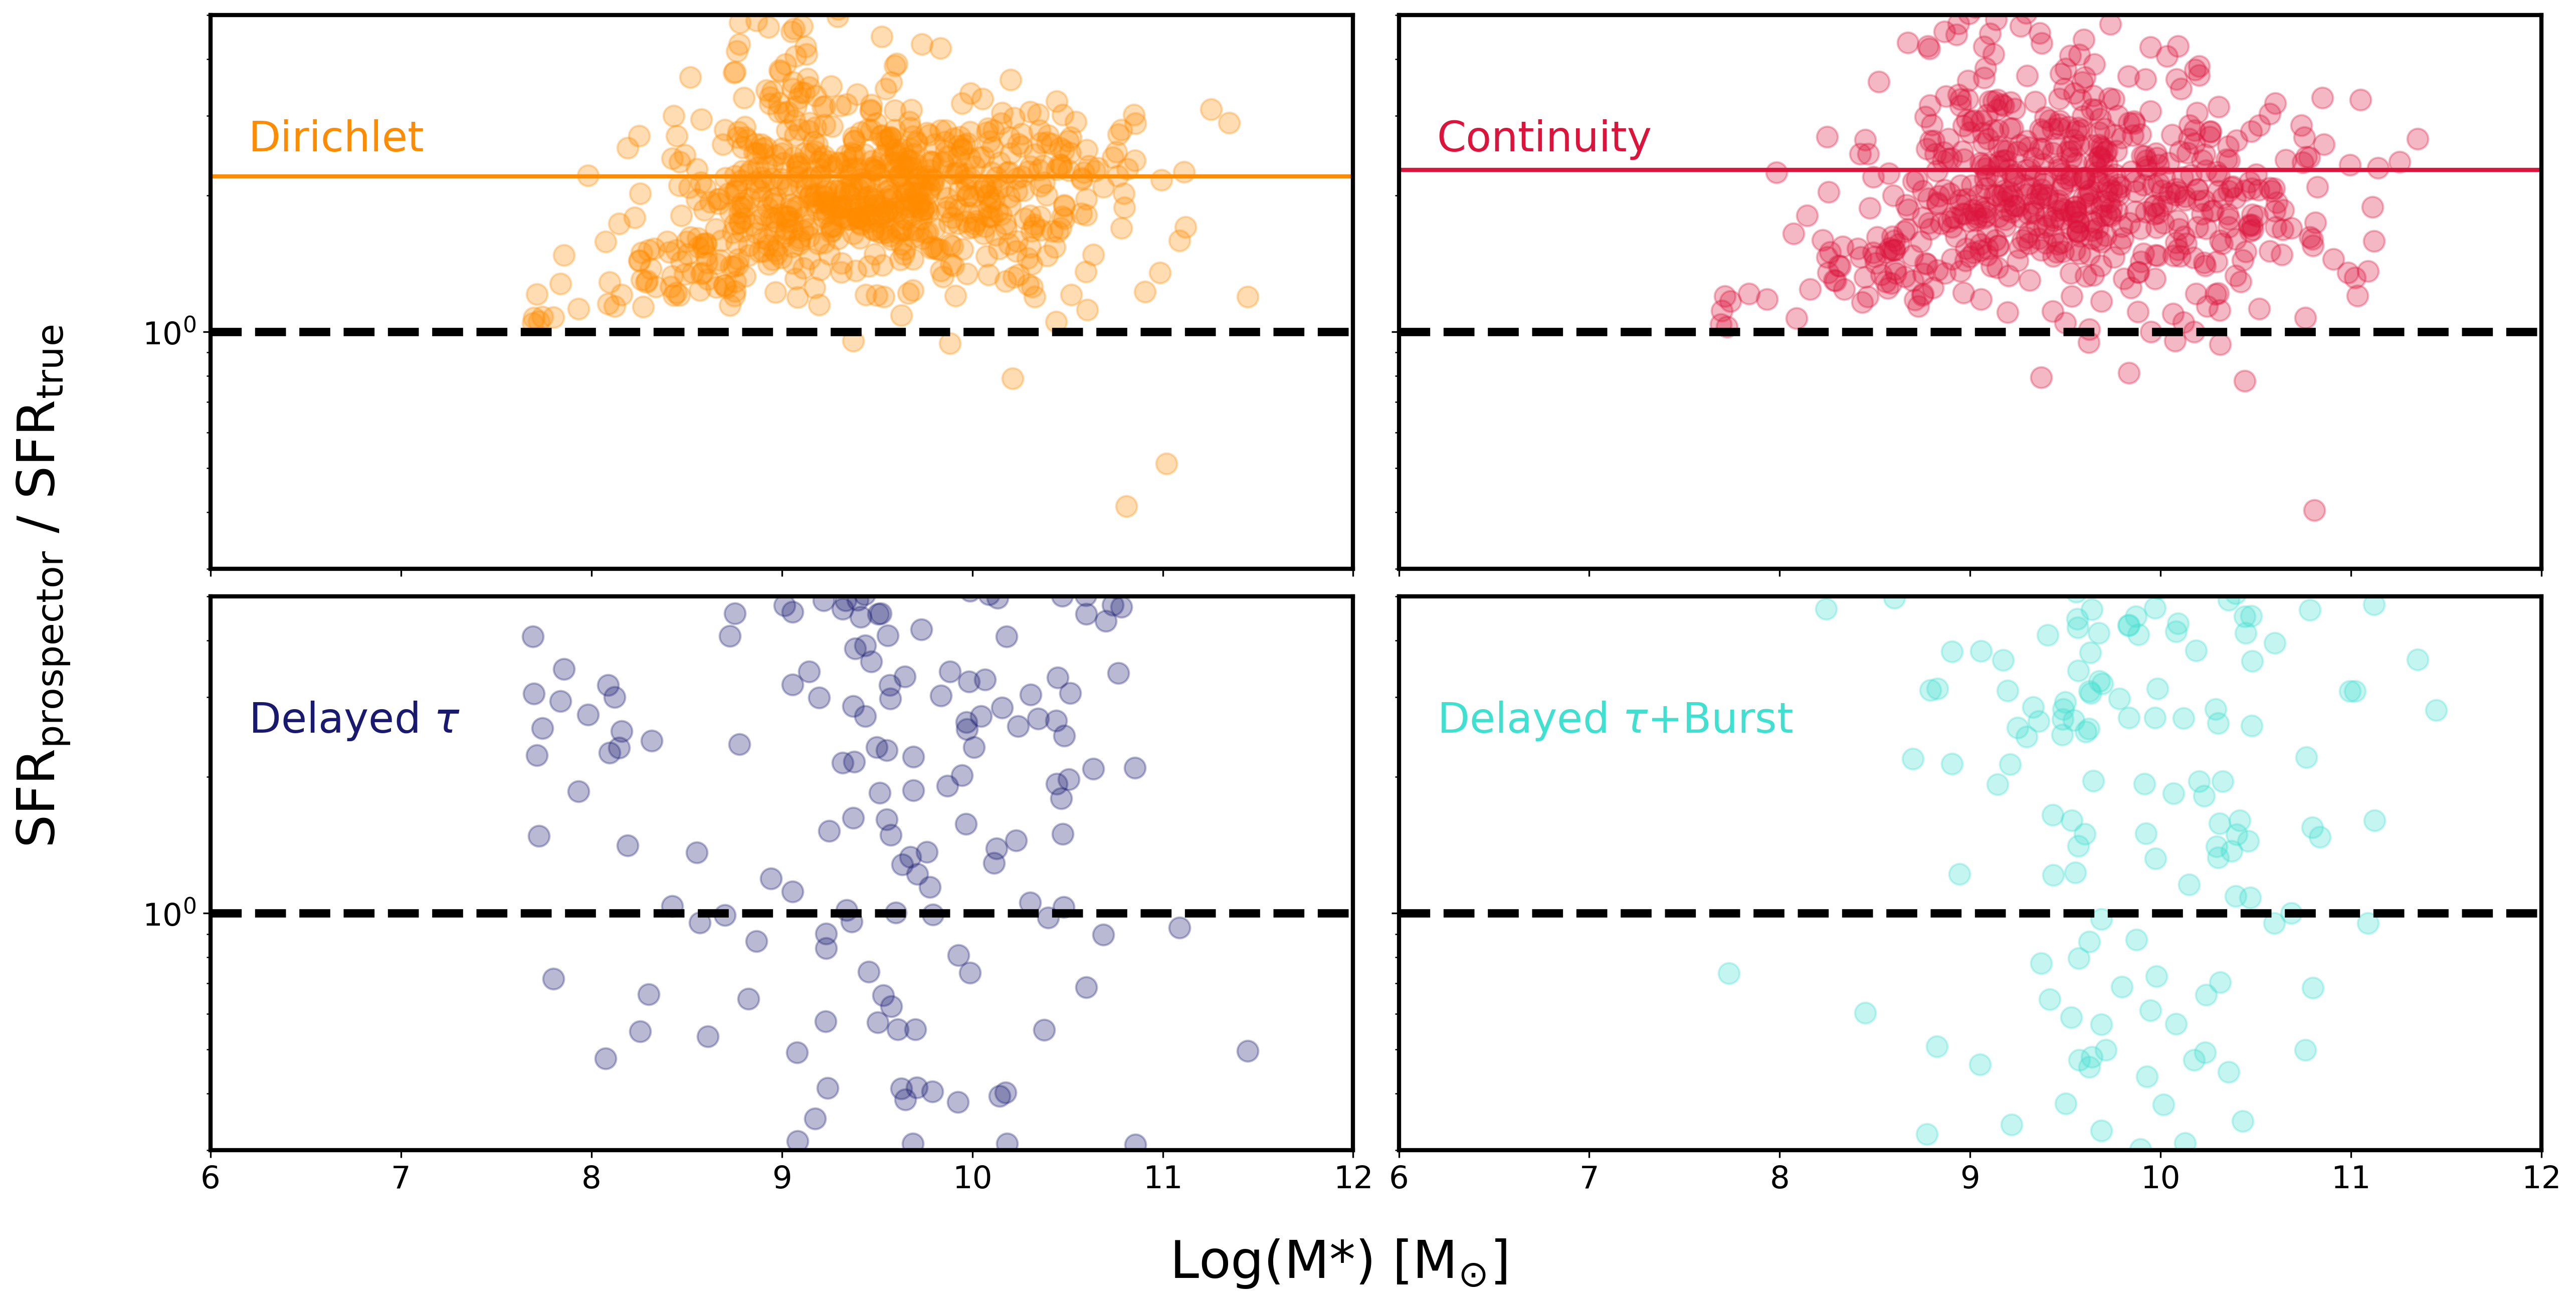
\includegraphics[width=.5\textwidth]{sfr_comp_grid_M.png}

\caption{Top: The ratio of \texttt{propsector} derived mass-weighted stellar ages to the true stellar ages. Bottom: The ratio of \texttt{prospector} derived star formation rates to the true star formation rates taken over the last 100 Myr. Solid lines denote the median of the ratios - the medians for both parametric SFR$_{100 \: \mathrm{Myr}}$ are at $\sim$ 2$\times$ 10$^{-2}$.}
\label{fig:age_sfr}

\end{figure}




\section{Discussion}

On average, the non-parametric SFHs outperform the parametric SFHs in all metrics, including estimation of stellar mass and age and star formation history recovery. At the minor expense of computation time, the more flexible SFHs are able to more accurately reconstruct the physical properties and growth history of galaxies. 


\subsection{Applications: recovering observed star forming main sequence}

We can use the stellar masses and star formation rates estimated with \texttt{prospector} to plot the star forming main sequence (SFMS) of our galaxies. The relation between these two properties is dependent on the ability of the SFH models to recover the correct SFH overall (and thus the stellar mass formed) and also the late time star formation rate over the last 100 Myr. Although from an observation point of view, the SFR is typically measured with star formation tracers (i.e. FIR luminosity, H$\alpha$ line flux), the SFR averaged over the last 100 Myr of the SFH estimated by SED modeling is still a useful property. Due to the exponentially declining nature of the two parametric SFH models used here, the late time SFR estimated from these models tends to be much lower than the true value. On the other hand, the late time SFR estimated from the non-parametric SFHs tends to overestimate the true SFRs, as seen in Figure \ref{fig:sfms}. However, the scatter in SFR$_{100 \: \mathrm{Myr}}$ for the non-parametric models is much less than that of the parametric models. Synthesizing these two results, the non-parametric SFHs are able to recover both the intrinsic SFMS of galaxies and also match two observed relations from the literature (\cite{boogaard_muse_2018}, \cite{schreiber_herschel_2015}). 

\subsection{Where the SFH models fail}


Although on average the non-parametric SFHs are able to recover the true stellar masses with great accuracy, there are some galaxies whose estimated properties do not agree at all with the true properties. As seen from the distribution in Figure \ref{fig:mass_comp}, the continuity SFH struggles with systematic underestimation, especially at the middle to lower mass end (M* $<$ 10$^{9.5} M_{\odot}$). Both non-parametric SFHs also appear to struggle with the high mass end, but the lack of high mass galaxies (M* $>$ 10$^{11.5} M_{\odot}$) does not allow for statistically meaningful results to be gleaned from these failures. 

Wholesale conclusions are difficult to draw as to the reason why the SFH models fail, as the reason may be unique for each galaxy. Looking to the plots comparing the estimated stellar ages and star formation rates to the true values reveal that although the scatter is much smaller for the non-parametric models as compared to the parametric models (owing to the on average increase in accurate stellar masses), we can see that the scatter tends to increase at the high mass end for both properties. Considering the degeneracy between the age of a galaxy and the degree of reddening stellar light experiences due to dust attenuation, we could expect the older, more massive systems to suffer from greater uncertainty when estimating stellar masses. Intuitively, poor estimates for stellar mass and stellar age originate from poor fits for the galaxy's SFH, as the shape of the SFH will affect the stellar ages but the overall normalization will affect the prediction for the amount of stellar mass formed. Practically, this means that SFHs that are lower than the true SFH on average will predict stellar masses that are smaller than the true values. The question then becomes \textit{why did the star formation histories fail to match the true values in some cases}? 

\begin{figure}[h!]

\centering
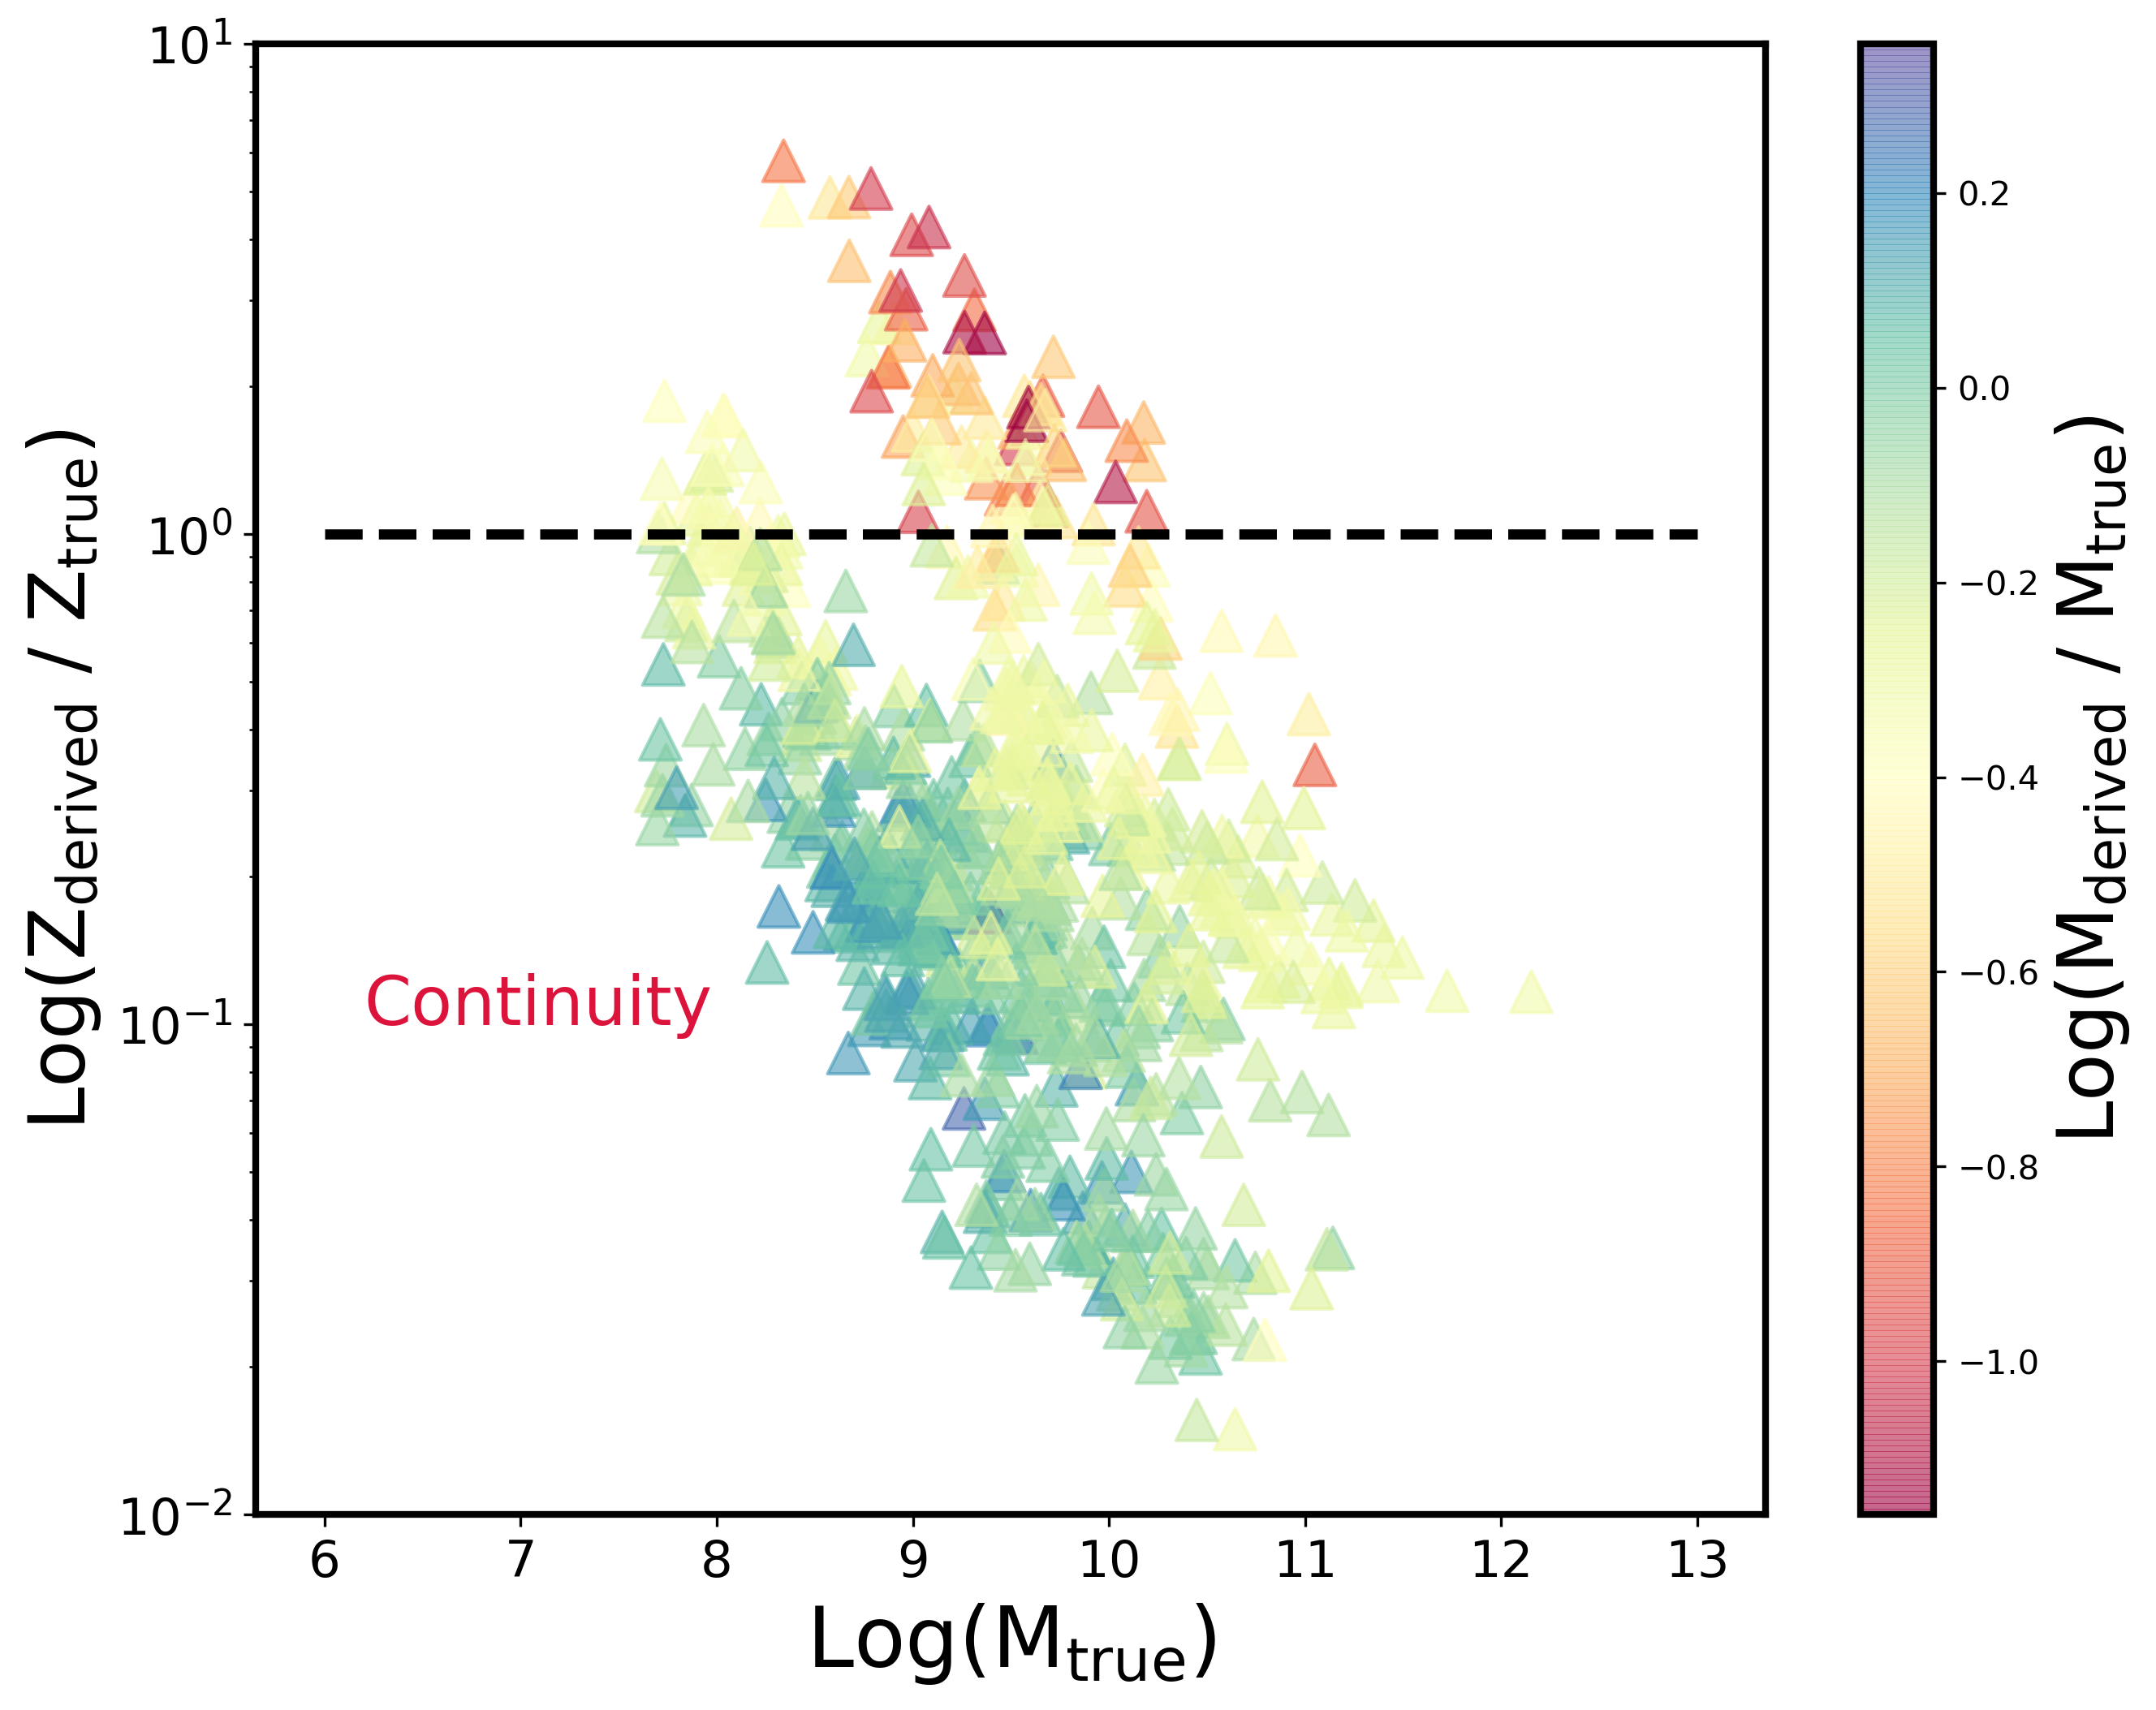
\includegraphics[width=0.47\textwidth]{Zratio_cont.png}\hfill
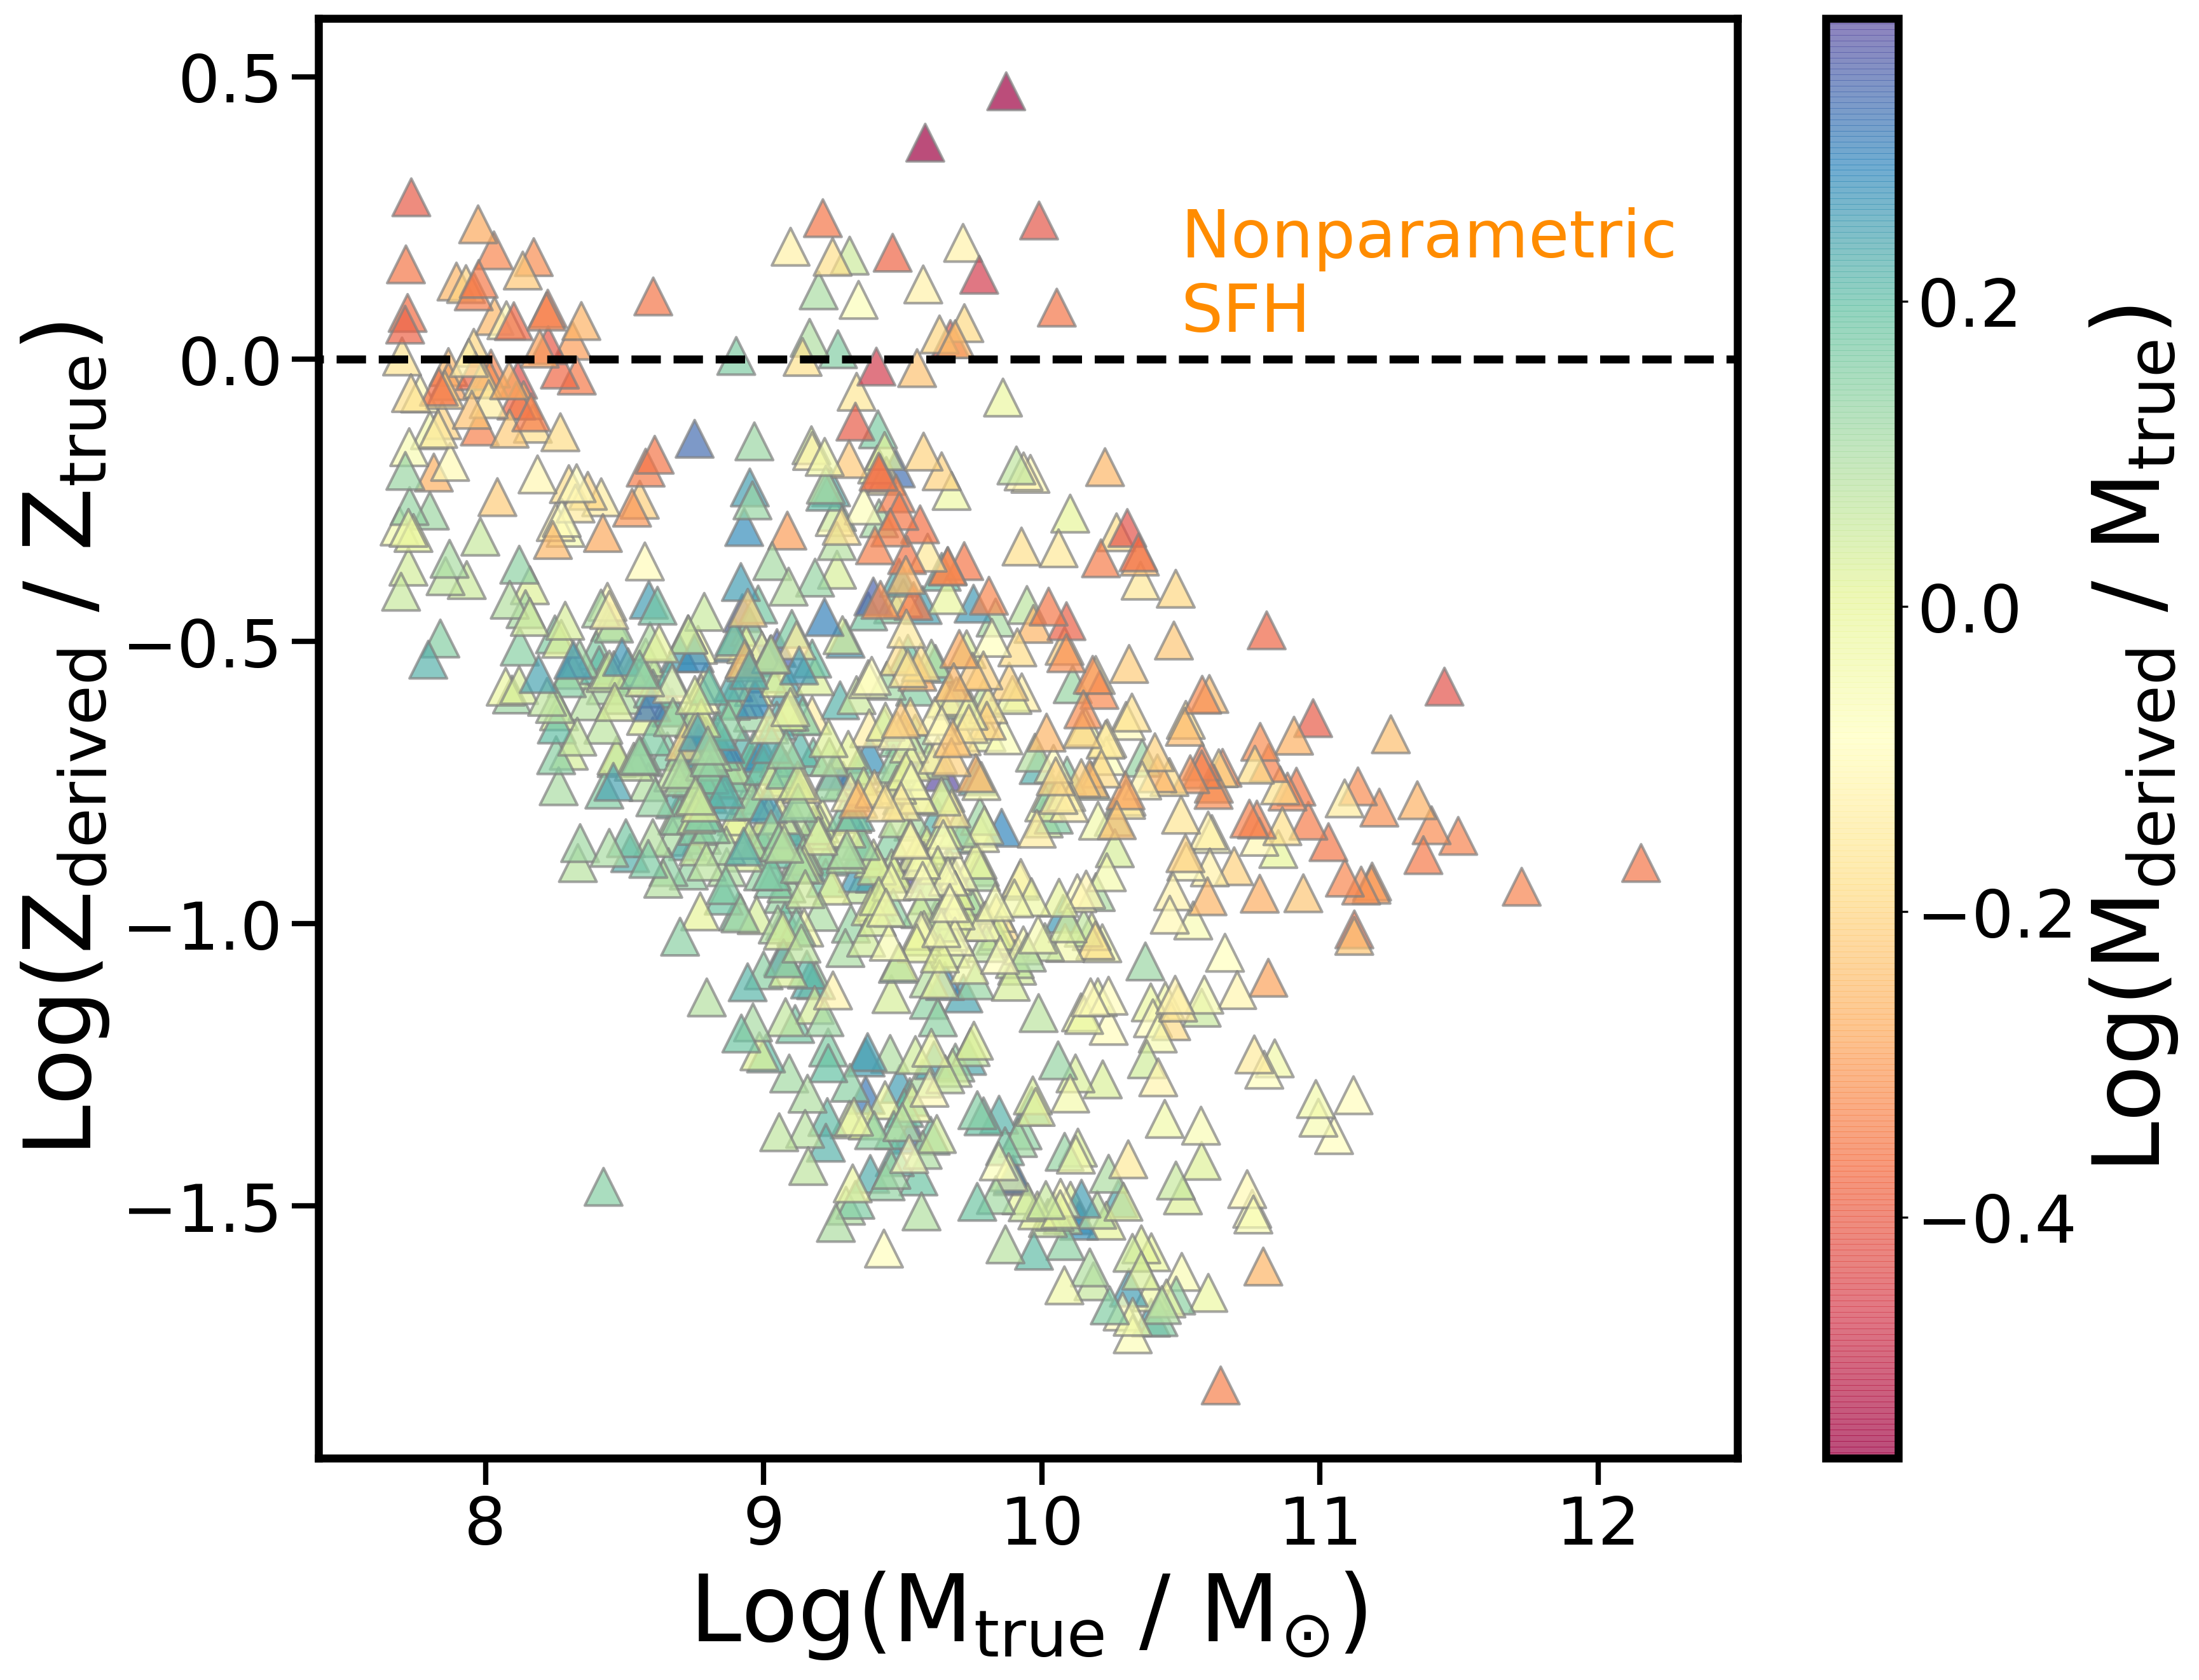
\includegraphics[width=0.47\textwidth]{Zratio_dir.png}

\caption{Correlation between the uncertainty in the predicted stellar metallicity and the uncertainty in the predicted stellar mass for the two non-parametric models. Points are color coded according to the ratio of predicted stellar mass to true stellar mass.}
\label{fig:zratio}
\end{figure}

One clue is from looking towards the metallicity. Prior to implementing the \cite{gallazzi_ages_2005} stellar mass - stellar metallcity prior, we instead used a uniform prior on the stellar metallcity. This allowed the metallicity to be fit without any regard to the predicted mass of the galaxy, a model which may not align with the processes happening within true galaxies. We discovered that the metallicities were being severely underestimated when compared to the true values. A caveat here, though, is that \texttt{prospector} estimates the light-weighted metallicity of the galaxy whereas the true metellicities for the \texttt{simba} galaxies are mass-weighted. Even so, light-weighted metallicities are typically higher than mass-weighted metallicities as the light is dominated by the newer generations of stars. The effect of small metallicities on a galaxy's SED is an increase in the UV flux, as low metallicity stars have less metals in their atmospheres to absorb light, and thus more UV photons can escape than with stars of solar metallicity. We found that in order to get a best fit SED and best fit stellar mass, \texttt{prospector} was forcing the stellar metallicities to very small values, a sign that some other model proponent was unable to match the observations. Namely, it seemed that the dust attenuation model was a poor match to the true attenuation and was forcing the metallicity down to compensate. We implemented the \cite{gallazzi_ages_2005} mass-metallicity prior to alleviate these model mismatches. Instead we found another trend: for galaxies whose stellar mass was underestimated, there existed a conspiracy between the model attenuation curve, stellar metallicity, and recent star formation, resulting in over estimations for all three properties. For example, the galaxy with the most underestimated stellar mass fit with the continuity SFH model had a moderately overestimated stellar metallicity, a severely overestimated dust attenuation curve, and a very high late time star formation episode coupled with severely underestimated SFRs overall. In effect, the moderately large metallicity and large amounts of dust attenuation offset the excess of UV flux from the high SFR over the past 100 Myr.  This resulted in a stellar mass approximately 14$\times$ smaller than the true value. The posteriors for all parameters were also much wider than average, indicating \texttt{dynesty}'s struggle to converge an SED fit. As a note, the vast majority of SEDs were reasonably well fit, even in the cases of poor predictions of physical properties, highlighting the necessity to use MCMC or similar algorithms to explore the entirety of the parameter spaces available as many combinations of different model parameters can result in similar SEDs. 

\begin{figure*}[h]

\centering
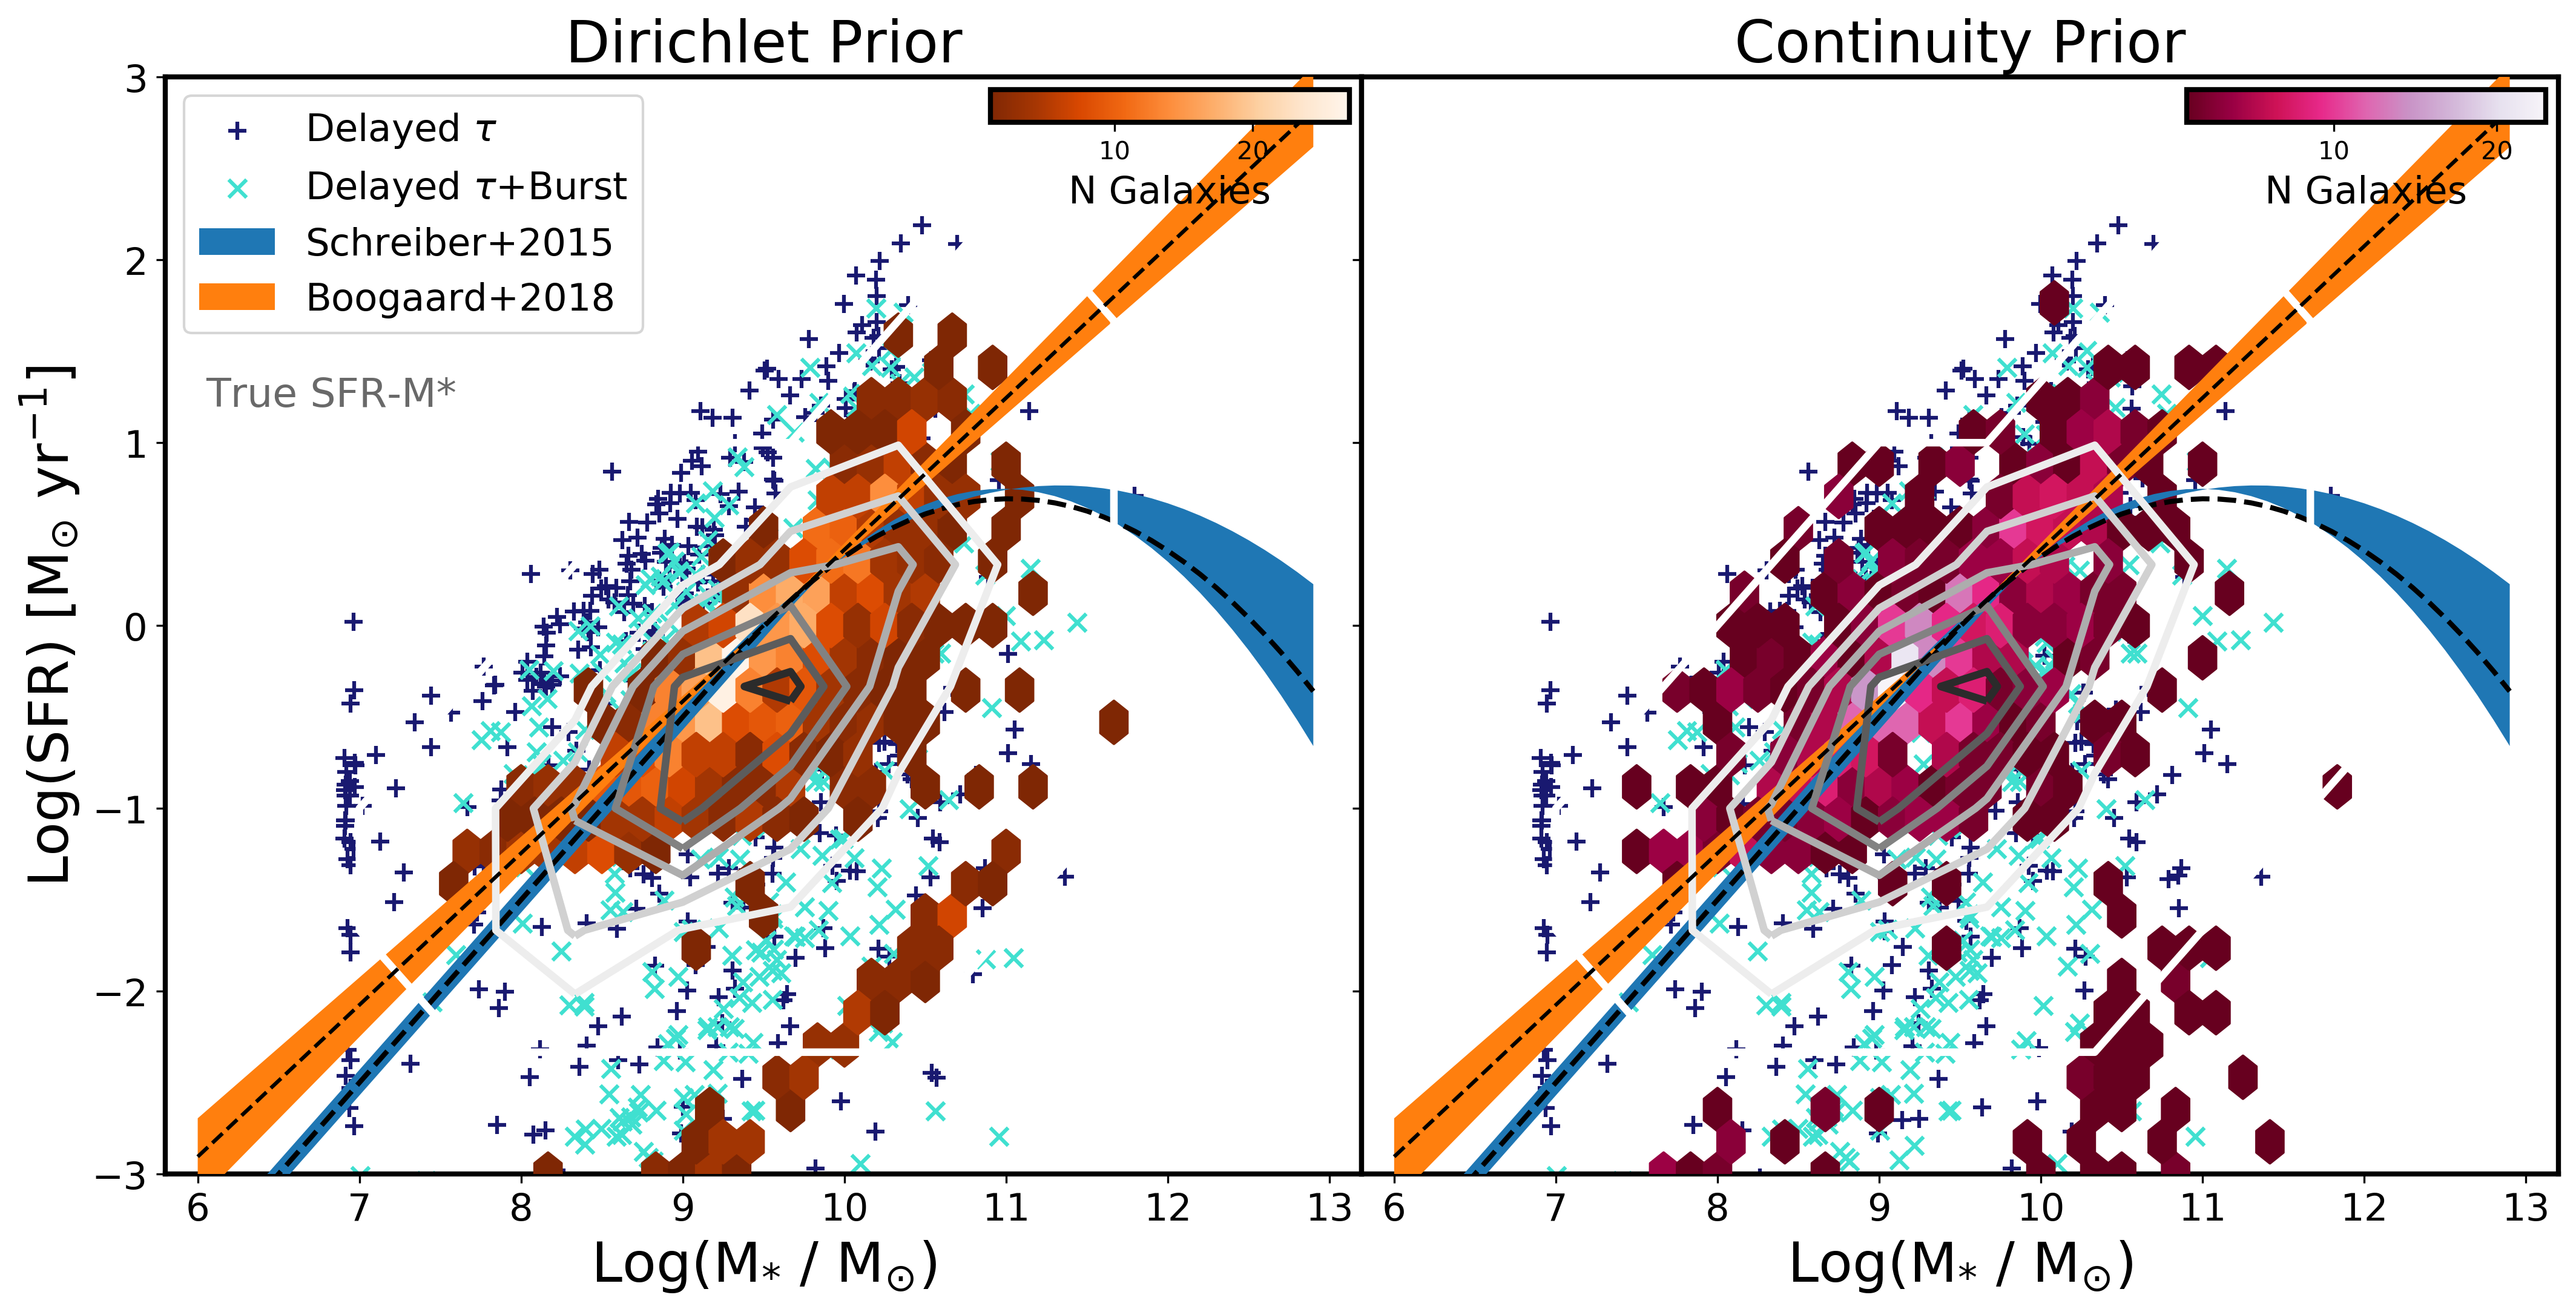
\includegraphics[width=\textwidth]{MS.png}\hfill

\caption{The star forming main sequence as estimated from \texttt{prospector}. Star formation rates are averaged over the last 100 Myr of the star formation history. The values estimated with the parametric SFHs are seen in the blue symbols. Those estimated with the non-parametric SFHs are seen in the hexbins. The intrinsic SFMS is seen in the gray contours. Two observations from the literature are shown for comparison.}
\label{fig:sfms}
\end{figure*}

We see the strong trend between the uncertainity in stellar metallicity and the uncertainity in stellar mass mentioned above and seen in Figure \ref{fig:zratio}. If \texttt{prospector} under estimates the stellar metallicity, the stellar mass is over estimated and conversely for over estimations of stellar metallicity. We see this trend for both models of non-parametric SFHs. Similar correlations with the mass-weighted stellar age and recent star formation rate are are not as strong, which can lead to the conclusion that the predicted stellar mass depends heavily on the metallicity. However, it seems more likely that the metallicity uncertainty can be attributed to uncertainty in the dust attenuation model. Dust attenuation primarily affects the UV light of a galaxy, so in the event that the modeled UV SED is incorrect, the metallicity can be forced to certain values to compensate. 

Importantly, it seems that modeling the SFH of a galaxy as flexible as possible is not enough to capture the physical processes governing galaxy evolution accurately enough so that the properties estimated from the modeled SED are also accurate. We can also model attenuation curves without a functional form so that the diversity in dust-star geometries seen in real galaxies can be accurately described. Further, we can attempt to constrain already existing model priors to values aligned with properties seen in state of the art cosmological simulations, which may alleviate the degeneracies still plaguing SED fitting described above. 




\section{Conclusions}

We have used simulated galaxies from the \texttt{simba} cosmological simulation to ground-truth the results of non-parametric SFHs used in SED modeling with \texttt{prospector}. These SFHs are more flexible in their ability to describe galaxy SFHs, which result in more accurate stellar mass and age estimates. We have shown that the uncertainty in stellar mass estimates decreases with the use of non-parametric SFHs, falling below a factor of 2 uncertainty, specifically with the Dirichlet non-parametric SFH. 

The importance of more accurate stellar mass estimates cannot be understated, as many galaxy scaling relations concerning galaxy formation and evolution include stellar mass. To this end, we showed we can recover the star-forming main sequence of our galaxies to a more accurate degree than with previous parametric SFHs, matching both the intrinsic SFMS and observed galaxies from the literature. However, these SFH models do not come without faults. We attempted to understand the cause of failed stellar mass predictions (an important note is that the 'failure' rate of the non-parametric SFHs is much less than the failure rate of the parametric models). Degeneracies between other properties and model parameters, specifically dust attenuation and stellar metallicity, and late time star formation rates can skew the stellar mass predictions away from the true values. The difficulty lies in the fact that the star formation history is only moderately constrained by broadband photometry so priors must be carefully implemented to allow a diverse range of SFHs to be modeled while simultaneously alleviating the degeneracy between other model parameters. Cosmological simulations can play an important role in future work to constrain priors not only for SFHs but also dust attenuation laws. We can also develop non-parametric models for dust attenuation in a similar way but the increase in computational resources and model degeneracies warrant caution. As such, we hope to explore further improvements to modeling SEDs and deriving physical properties from broadband photometry.  



\bibliographystyle{aasjournal}
\bibliography{bib2}{}




\end{document}


